\chapter{Investigation of 3D Printing Filament}
\renewcommand{\baselinestretch}{\mystretch}
\label{chap:Invest}
%\setlength{\parindent}{0pt}

\section{Methodology}
After the fabrication of the filament, it is essential to investigate its 3D-printability property. Two CAD models were designed to print for different reasons. One was the standard cube and the other one was the waveguide.
\subsection{Cube printing}
Our extrusion of ABS and pumice did not use the same weight of materials that measured before combination since there must be some materials left in the coffee grinder, the hopper and even in a screw. It is not reliable to judge the weight percentage by weighting materials before all procedure. The standard cube may give the information about the density of the printing filament indirectly by weighing it. Then it is possible to deduce the weight percentage of pumice in the new material since the density of ABS and pumice powder are known.\\ 
\begin{figure}[htbp]
  \centering
  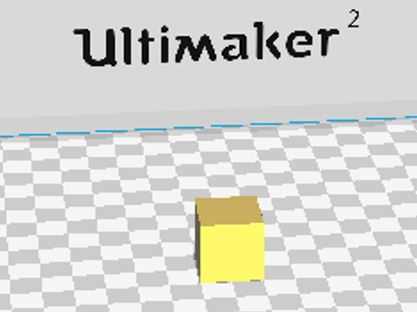
\includegraphics[height=6.5cm,width=10cm]{Figs5//cube_design.JPG}
  \caption[The cube design in Cura]{\footnotesize The cube design in Cura.}
  \label{Fig:cube}
\end{figure}
\subsection{Waveguides printing}
The main task is to print the waveguides with different materials and test their mechanical precision. In particular, it attracted our attention that the roughness of the inner walls of the waveguides which contribute to their performance in practice\cite{d20153}. The waveguides printed with different materials could help us to judge the potential of these materials and find the influences of adding pumice powder to ABS pellets.

\begin{figure}[htbp]
  \centering
  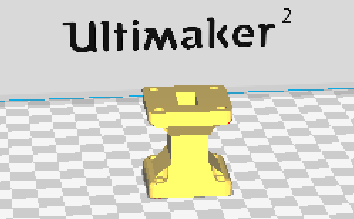
\includegraphics[width=10cm]{Figs//waveguide_design.PNG}
  \caption[The cube design in Cura]{\footnotesize The waveguide design in Cura.}
  \label{Fig:waveguide}
\end{figure}

\section{Experiment}
It is quite frustrated to use pure ABS filament in 3D printer due to the warp of ABS and the difficulties on bed adhesion. There are lots of tips and parameter settings in experiment required to investigate.
\subsection{Design in Cura}
Cura is a multi-functional slicing software that can slice any 3D designs into layers and save the file as G-Code, which could be recognised by the 3D printer. This G-Code file as a text document contains a list of commands for the 3D printer to understand and work with, such as print this part with a speed and print another part with another speed etc. In the Cura software, there are several settings for 3D printing that worth investigating.
\begin{itemize}
\item Printing speed
\end{itemize}
It should be noted that the printing speed has a big influence on the printing quality. In extruding process, the extruding speed is based on the extruding temperature. The print speed should compile with the extruding temperature. The Ultimaker 2 printer has these settings. \\
\\
As for the meaning of speed setting in the Cura software, there is an opportunity to tune the printing speed for different parts of the print. In general, the print speed could be set to 50mm/s and travel speed was 100 mm/s for maximum quality. The initial layer speed should be the lowest one which is 30\% of the print speed for good bed adhesion. The improvements that can be made in Cura are the specific sub-settings of print speed, including infill speed, outer/inner wall speed, top/bottom speed and support speed as Figure\ref{Fig:speed} describes. It is better to slow down the outer wall speed and top/bottom speed as well.
\begin{figure}[htbp]
  \centering
  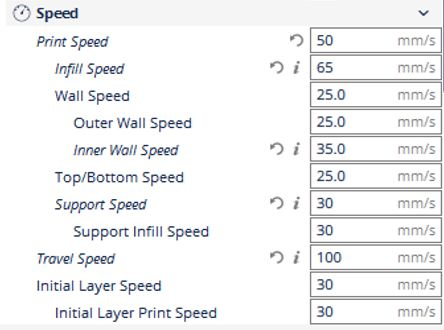
\includegraphics[scale=0.8]{Figs5//speed.JPG}
  \caption[The speed settings in Cura]{\footnotesize The speed settings in Cura.}
  \label{Fig:speed}
\end{figure}

\begin{itemize}
\item Thickness of walls
\end{itemize}
The settings of the shell (i.e. wall thickness and top/bottom thickness) affect the mechanical strength of the printed component. For instance, the 1mm wall thickness makes the waveguides fragile in the middle part while 3mm wall thickness offers the strong body. In general, the sufficient wall thickness setting is 2 or 3 times of the line width. 
\begin{figure}[t] % make the image in the middle of paragraph
	\centering
	\subfigure[]{
    \begin{minipage}[t]{0.4\textwidth}
			\centering
			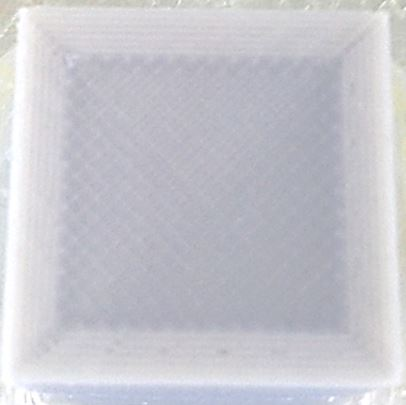
\includegraphics[height=5cm]{Figs5//thickness2.JPG}
		\end{minipage}
	}
	\subfigure[]{
		\begin{minipage}[t]{0.4\textwidth}
			\centering
			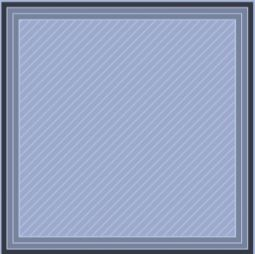
\includegraphics[height=5cm]{Figs5//thickness.jpg}
		\end{minipage}
	} 

  \caption[The setting of wall thickness]{\footnotesize The setting of wall thickness:(a)3mm, (b)3 times of the line width. }
  \label{Fig:thickness}
\end{figure}

\begin{itemize}
\item Infill density
\end{itemize}
Infill is also a significant parameter for 3D printed components. It would cause the warp of ABS if there are lots of solid layers with light infill at the bottom. To be specific, the warp stems from the rapid cooling of the material so that the variety of infill density should be avoided. Since the wall thickness has been decided, the only way to increase the change of infill is using 100$\%$ infill for waveguides printing after several investigations. In Figure\ref{Fig:infill}, it could be shown that the warp of ABS bring the imperfection of the infill part printing while 100$\%$ infill density avoided it. And it needs more material for printing.
\begin{figure}[htbp] % make the image in the middle of paragraph
	\centering
	\subfigure[]{
    \begin{minipage}[t]{0.4\textwidth}
			\centering
			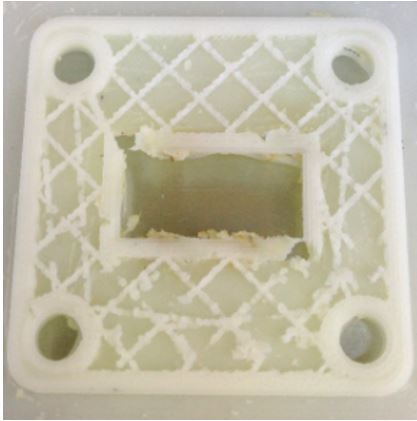
\includegraphics[height=5.5cm]{Figs5//infill1.JPG}
		\end{minipage}
	}
	\subfigure[]{
		\begin{minipage}[t]{0.4\textwidth}
			\centering
			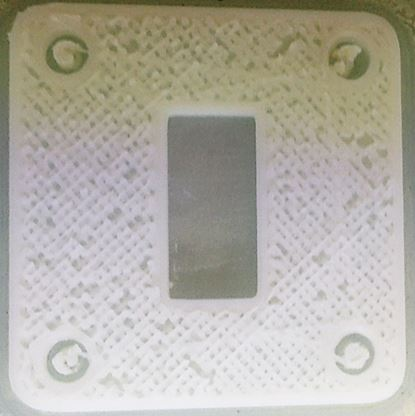
\includegraphics[height=5.5cm]{Figs5//infill2.JPG}
		\end{minipage}
	} 
	\subfigure[]{
		\begin{minipage}[t]{0.4\textwidth}
			\centering
			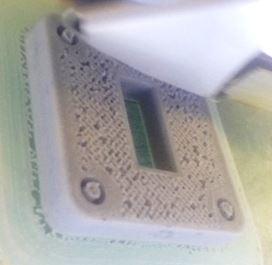
\includegraphics[height=5cm]{Figs5//infill4.JPG}
		\end{minipage}
	} 
	\subfigure[]{
		\begin{minipage}[t]{0.4\textwidth}
			\centering
			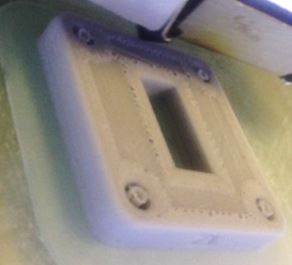
\includegraphics[height=5cm]{Figs5//infill5.JPG}
		\end{minipage}
	} 

  \caption[The settings of the infill density]{\footnotesize The settings of the infill density:(a)30$\%$, (b)80$\%$, (c)80$\%$, (d)100$\%$. }
  \label{Fig:infill}
\end{figure}

\begin{itemize}
\item Support structure
\end{itemize}
There are several patterns for support structure in Cura. The best solution depends on your 3D model and the requirements of support part. The support density also should be taken into consideration. Another parameter is Z distance which means the distance from the bottom and top of the support structure to the main printed model. These settings requires delicate designs. As a trade-off, the support structure should be strong but easy to remove. Finally, we have chosen 25$\%$ concentric support structure to print good waveguides. 
\begin{figure}[htbp] % make the image in the middle of paragraph
	\centering
	\subfigure[]{
    \begin{minipage}[t]{0.32\textwidth}
			\centering
			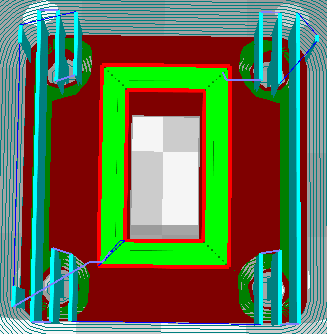
\includegraphics[height=5cm]{Figs5//lines.PNG}
		\end{minipage}
	}
	\subfigure[]{
		\begin{minipage}[t]{0.32\textwidth}
			\centering
			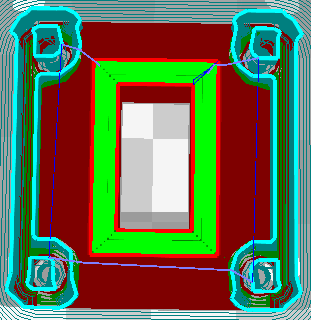
\includegraphics[height=5cm]{Figs5//concentric.PNG}
		\end{minipage}
	} 
 
 \subfigure[]{
		\begin{minipage}[t]{0.31\textwidth}
			\centering
			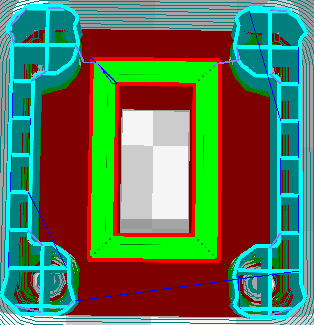
\includegraphics[height=5cm]{Figs5//geid.PNG}
		\end{minipage}
	} 
     \subfigure[]{
		\begin{minipage}[t]{0.3\textwidth}
			\centering
			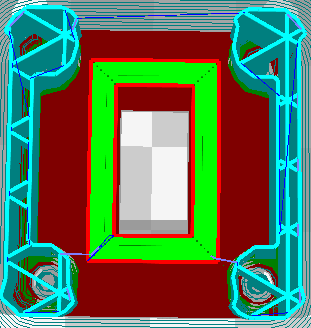
\includegraphics[height=5cm]{Figs5//triangles.PNG}
		\end{minipage}
	} 
     \subfigure[]{
		\begin{minipage}[t]{0.3\textwidth}
			\centering
			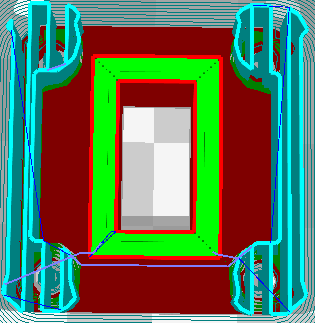
\includegraphics[height=5cm]{Figs5//zigzag.PNG}
		\end{minipage}
	} 
  \caption[Support patterns]{\footnotesize Support patterns (a)line, (b)concentric, (c)grid, (d)triangles, (e)Zig Zag. }
  \label{Fig:support}
\end{figure}

\begin{itemize}
\item Brim
\end{itemize}
The brim is a nice feature in Cura software to add a single layer flat area around the base of the object, which could decrease the probability of warping. Brim increases the bottom layer area so that it is beneficial to bed adhesion, especially the flatness of the corners.  when printing completes, it could be removed easily. In our experiment, the width of Brim does not make big differences as Figure \ref{Fig:Brim} suggests.
\begin{figure}[htbp] % make the image in the middle of paragraph
	\centering
	\subfigure[]{
    \begin{minipage}[t]{0.45\textwidth}
			\centering
			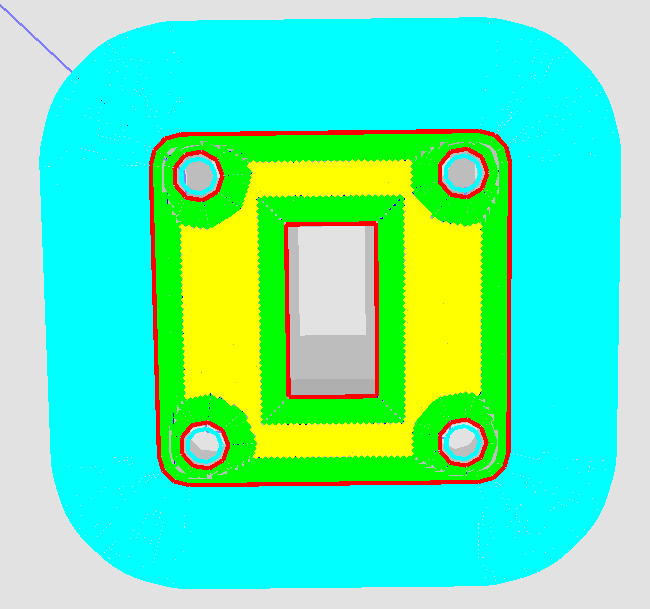
\includegraphics[height=6cm]{Figs5//10mmbrim.PNG}
		\end{minipage}
	}
	\subfigure[]{
		\begin{minipage}[t]{0.45\textwidth}
			\centering
			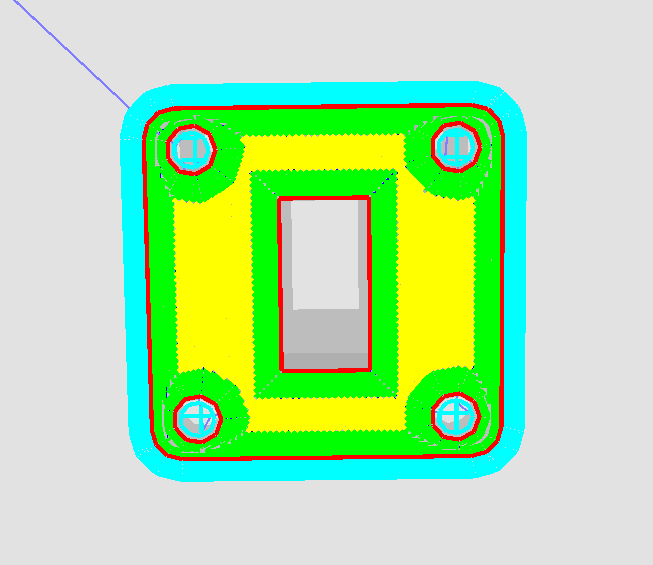
\includegraphics[height=6cm]{Figs5//2mmbrim.PNG}
		\end{minipage}
	} 

  \caption[The brim thickness]{\footnotesize The brim thickness of (a)10mm, (b)2mm. }
  \label{Fig:Brim}
\end{figure}

\subsection{Tunable components in UM2}
After finishing the designs in the computer, it is more flexible to adjust some settings in the 3D printer. Some of them should be decided before the printing start while others could be changeable during the printing process\cite{stick}.

\begin{itemize}
\item Bed levelling
\end{itemize}
As the name describes, bed levelling is to make sure that the build plate is completely level. In Ultimaker 2, this work belongs to the maintenance operation. When you level your plate, the distance between nozzle head and the plate is also adjusted.  As the UM2 instructs, a slice of paper was put between the nozzle head and the plate to judge the suitable nozzle distance if you feel a little friction when you remove the paper. In this way, the nozzle distance is about 0.1mm which is exactly the layer thickness. As can be seen in Figure\ref{Fig:bed}, the nozzle distance might be too close for material to come out of the nozzle and adhere evenly or be too far away for material to stick to the bed properly. Therefore, the bed levelling results in the good quality of the first layer.

\begin{figure}[htbp] % make the image in the middle of paragraph
	\centering
	\subfigure[]{
    \begin{minipage}[t]{0.5\textwidth}
			\centering
			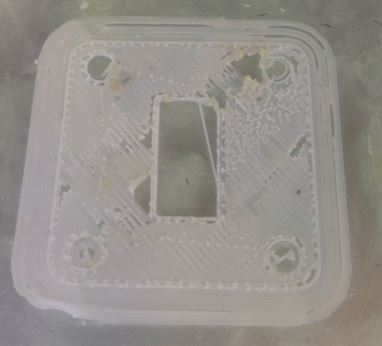
\includegraphics[height=6cm]{Figs5//bad_first_layer.JPG}
		\end{minipage}
	}
	\subfigure[]{
		\begin{minipage}[t]{0.45\textwidth}
			\centering
			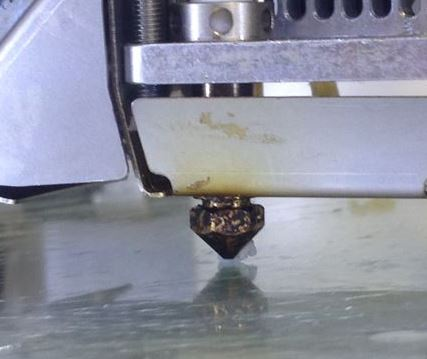
\includegraphics[height=6cm]{Figs5//bad_adhesion1.JPG}
		\end{minipage}
	} 

  \caption[The distance between nozzle head and build plate]{\footnotesize The distance between nozzle head and build plate is (a)too close, (b)too far.}
  \label{Fig:bed}
\end{figure}

\begin{itemize}
\item Utilization of fans
\end{itemize}
Ultimaker 2 has dual fans for cooling down the extruded material. However, it is mentioned in chapter three that the fans may bring the instability for ABS extrusion. As for bed adhesion, the use of fans has the warping or splitting effect when printing with the ABS filament. Therefore, the fans are not utilised in the experiment. And our 3D printer is placed in a small room other than under the air-conditioner in order to avoid these influences as well.
\begin{figure}[htbp]
  \centering
  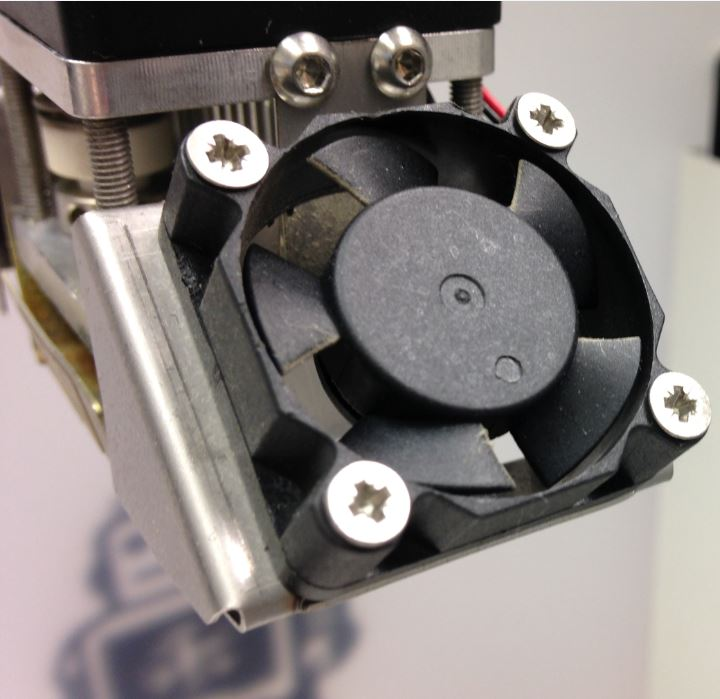
\includegraphics[scale=0.4]{Figs5//fan.JPG}
  \caption[The fan installed in UM2]{\footnotesize The fan installed in UM2}
  \label{Fig:fan}
\end{figure}

\begin{itemize}
\item Tension of the feeder
\end{itemize}
There are some effects at the filament feeder that could indicate the extrusion problem. This problem often happens in the hot end, rather than the feeding part. During the experiment, the print fails sometimes since the filament is grinded by the knurled wheel of the feeder. There are two main reasons for this situation. One is that the nozzle head is blocked and the feeder does not give the enough strength to push the material.  The other one is that the filament diameter rapidly changes (shrinks or enlarges) so that the feeder's tension is not suitable for filament moving. Once the filament stops moving, it is easily grinded by the wheel and it never moves again. The solution to this problem is to replace the grinded filament from the Ultimaker 2 by a new piece of filament. It could waste the materials so the good setting at first is very important. The tension of the feeder should be the trade-off to give the enough strength to push the filament as well as not grind the filament.

\begin{figure}[htbp]
  \centering
  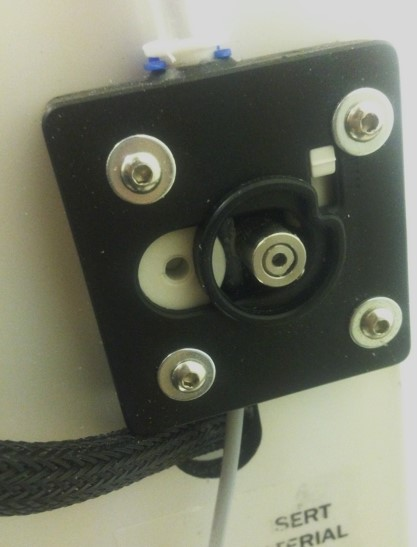
\includegraphics[scale=0.6]{Figs5//feeder.JPG}
  \caption[The filament is grinded by the feeder]{\footnotesize The filament is grinded by the feeder.}
  \label{Fig:feeder}
\end{figure}

\begin{itemize}
\item Build platform
\end{itemize}
The glass plate is a good choice for good bed adhesion of materials. As for ABS, it is also advised to heat the build platform to avoid the warping. This method could ensure that the first layer of the ABS does not cool down rapidly, which may result in the shrink of ABS. The recommended temperature of the build platform is from 90$^{\circ}$C to 110$^{\circ}$C.  According to some investigations on it, 105 $^{\circ}$C seems the best setting for our materials. \\
\\
It is also known that a bare glass plate cannot give the strong adhesion. Another tip is to apply a thin layer of glue on it. There are lots of choices of glue. The strongest adhesion will cause the difficulties in removing the products from the build plate while the lightest adhesion cannot meet the requirement. With these considerations, we have used the PVA-based glue stick. The glue is always applied on the cool build plate, It could be dried when heating the plate before printing.  When print was complete, it is easy to remove it after the bed is cooled down to the air temperature entirely and use a wet paper towel with hot water to clean the build platform. 
\begin{itemize}
\item Extruding temperature
\end{itemize}
It is quite tricky for extruding temperature setting. The high temperature could give you the fast extruding speed to some degree while it may bring the back-flow of the material since the ABS is too soft to push. And a lower extruding temperature would slow down the extrusion process. Moreover, the thickness of the layer may be decreased and there may be some gaps between each line. It means that the extruding speed cannot follow the print speed. The latter case could be dealt with by slow down the print speed. For safety, we set 240 $^{\circ}$C as the extruding temperature in the 3D printer. 
\begin{itemize}
\item Printing speed
\end{itemize}
In Ultimaker 2, the print speed could be tuned anytime during printing. The speed is controlled by the percentage of designed speed in Cura. For example, setting 50 mm/s print speed in Cura and 30$\%$ speed in UM2 offers 15mm/s as the true speed. It is an advantage of the printer that we can manually change the speed according to the performance rather than discard the print and start a new one.
\begin{figure}[htbp] % make the image in the middle of paragraph
	\centering
	\subfigure[]{
    \begin{minipage}[t]{0.45\textwidth}
			\centering
			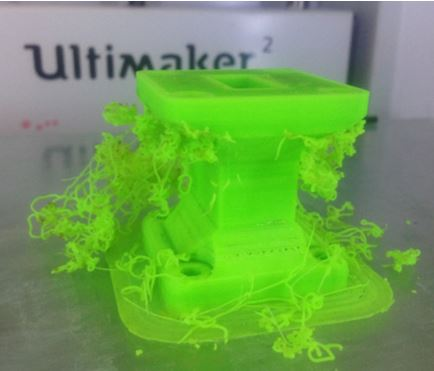
\includegraphics[height=6cm]{Figs5//speed1.JPG}
		\end{minipage}
	}
	\subfigure[]{
		\begin{minipage}[t]{0.45\textwidth}
			\centering
			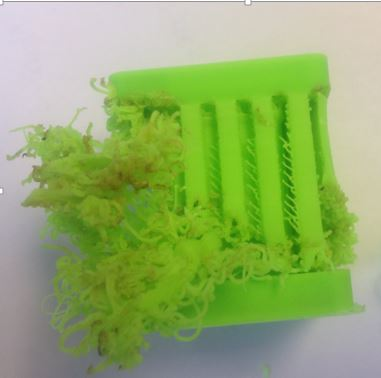
\includegraphics[height=6cm]{Figs5//speed2.JPG}
		\end{minipage}
        }
  \caption[The filament made with different speed]{\footnotesize The filament made with (a)70$\%$ speed, (b)50$\%$ speed. }
  \label{Fig:speed}
\end{figure}
\subsection{3D printing results}
The basic judgment of the success of the print is the first layer. If the first layer is sufficiently nice, we could continue to print all model otherwise we should change the settings and start a new one again. Figure \ref{Fig:first layer} offers the examples of first layers. And all of our produced filament could print a successful first layer in UM2.
\begin{figure}[htbp]
  \centering
  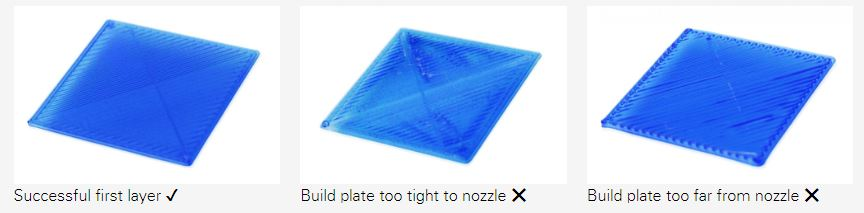
\includegraphics[scale=0.65]{Figs5//first_layer.JPG}
  \caption[The different situations of the first layer]{\footnotesize The different situations of the first layer.}
  \label{Fig:first layer}
\end{figure}
\begin{itemize}
\item Cubes
\end{itemize}
The infill setting of the cube is 100$\%$ due to its design aim that is to measure the density of the material. At first, we only print a 1 $cm^3/g$ to test the density of the filament. However, the result shows a big measure error and the printed cube is very irregular as Figure\ref{Fig:bad cube} represents. The volume of it is too small and the print settings including print speed wall thickness are not proper. In this case, an 8 $cm^3/g$ cube is more reasonable.
\begin{figure}[t]
  \centering
  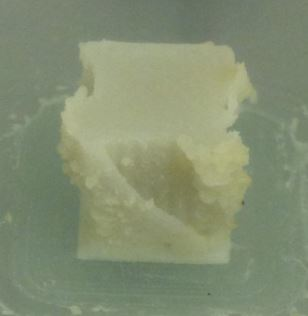
\includegraphics[scale=0.6]{Figs5//bad_cube.JPG}
  \caption[The 3D-printed 1 $cm^3/g$ cube]{\footnotesize The 3D-printed 1 $cm^3/g$ cube.}
  \label{Fig:bad cube}
\end{figure}
Since it is composed of lots of solid layers, the corners of it warp easily due to the different cooling speed of ABS at the corners. And there are air bubbles in the filament which result in the thinner layer than the printer suppose it to be. Therefore, the final results are still not good as shown in Figure \ref{Fig:cubes}. The weight of each cube is described in Table \ref{tab:cube density}. The density calculated by this measurement is really different from the theoretical one.
\begin{table}[htbp]
\centering
\caption {The weight and density of the printed cubes}
\begin{tabular}{c c c c}
\hline
\textbf{Weight} & \textbf{Material} & \textbf{Measured density} & \textbf{theoretical density}\\
\hline
7.00g & ABS with 0 wt.$\%$ pumice &  0.875 $g/cm^3$ &  1.030$g/cm^3$ \\
7.11g & ABS with 1 wt.$\%$ pumice & 0.889 $g/cm^3$ &  1.036$g/cm^3$  \\
6.48g & ABS with 2 wt.$\%$ pumice &  0.81 $g/cm^3$&  1.041$g/cm^3$  \\
6.86g & ABS with 3 wt.$\%$ pumice &  0.858 $g/cm^3$&  1.048$g/cm^3$  \\
6.45g & ABS with 4 wt.$\%$ pumice &  0.806 $g/cm^3$&  1.054$g/cm^3$  \\
6.94g & ABS with 5 wt.$\%$ pumice &  0.868 $g/cm^3$&  1.060$g/cm^3$  \\
6.60g & ABS with 6 wt.$\%$ pumice &  0.825 $g/cm^3$&  1.066$g/cm^3$  \\
\hline
\end{tabular}
\label{tab:cube density}
\end{table}

\begin{figure}[htbp] % make the image in the middle of paragraph
	\centering
	\subfigure[]{
    \begin{minipage}[t]{0.35\textwidth}
			\centering
			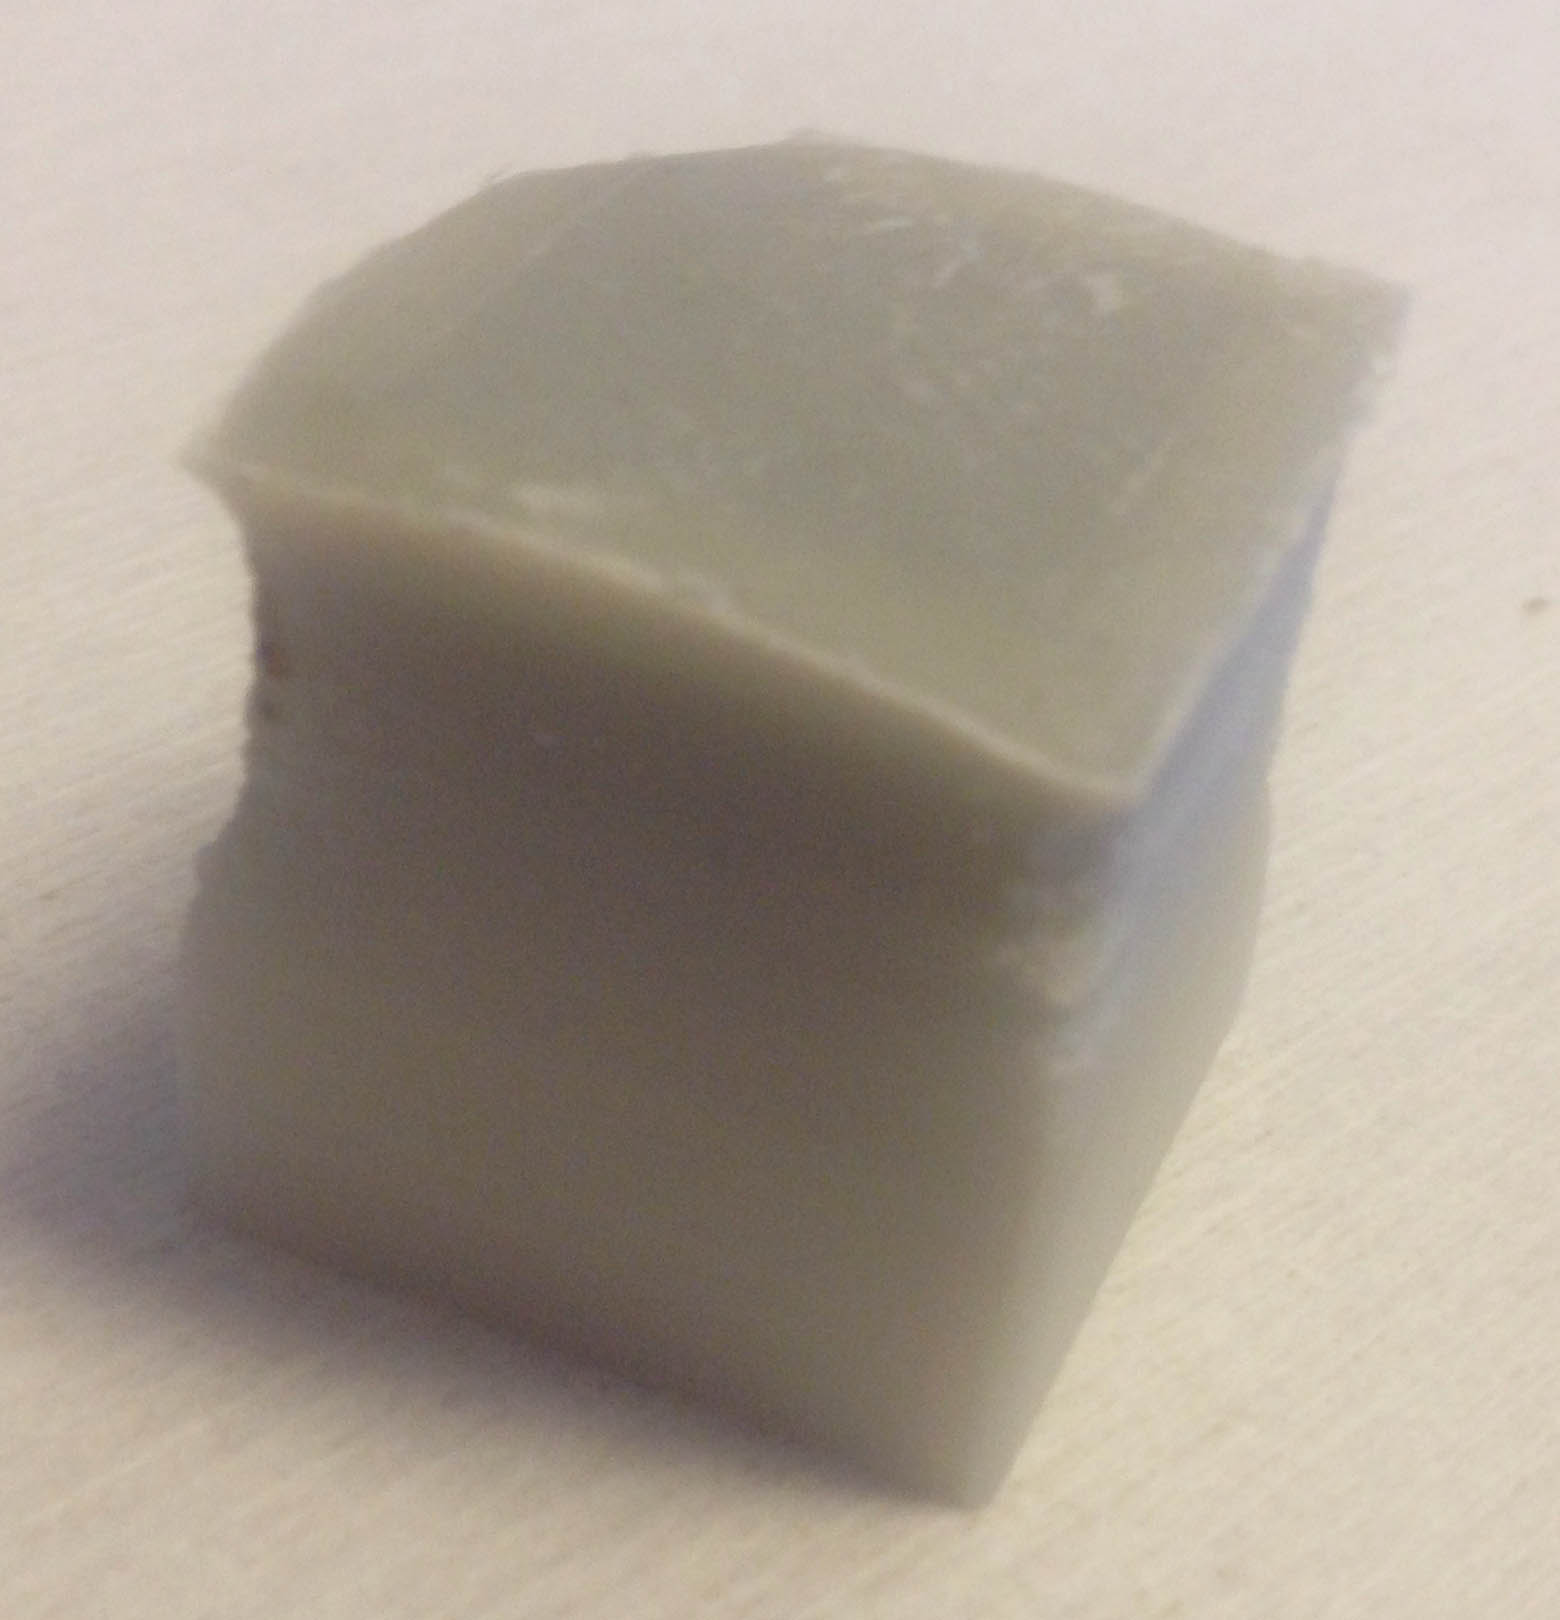
\includegraphics[height=4.6cm,width=4.6cm]{Figs5//0.JPG}
		\end{minipage}
	}
	\subfigure[]{
		\begin{minipage}[t]{0.35\textwidth}
			\centering
			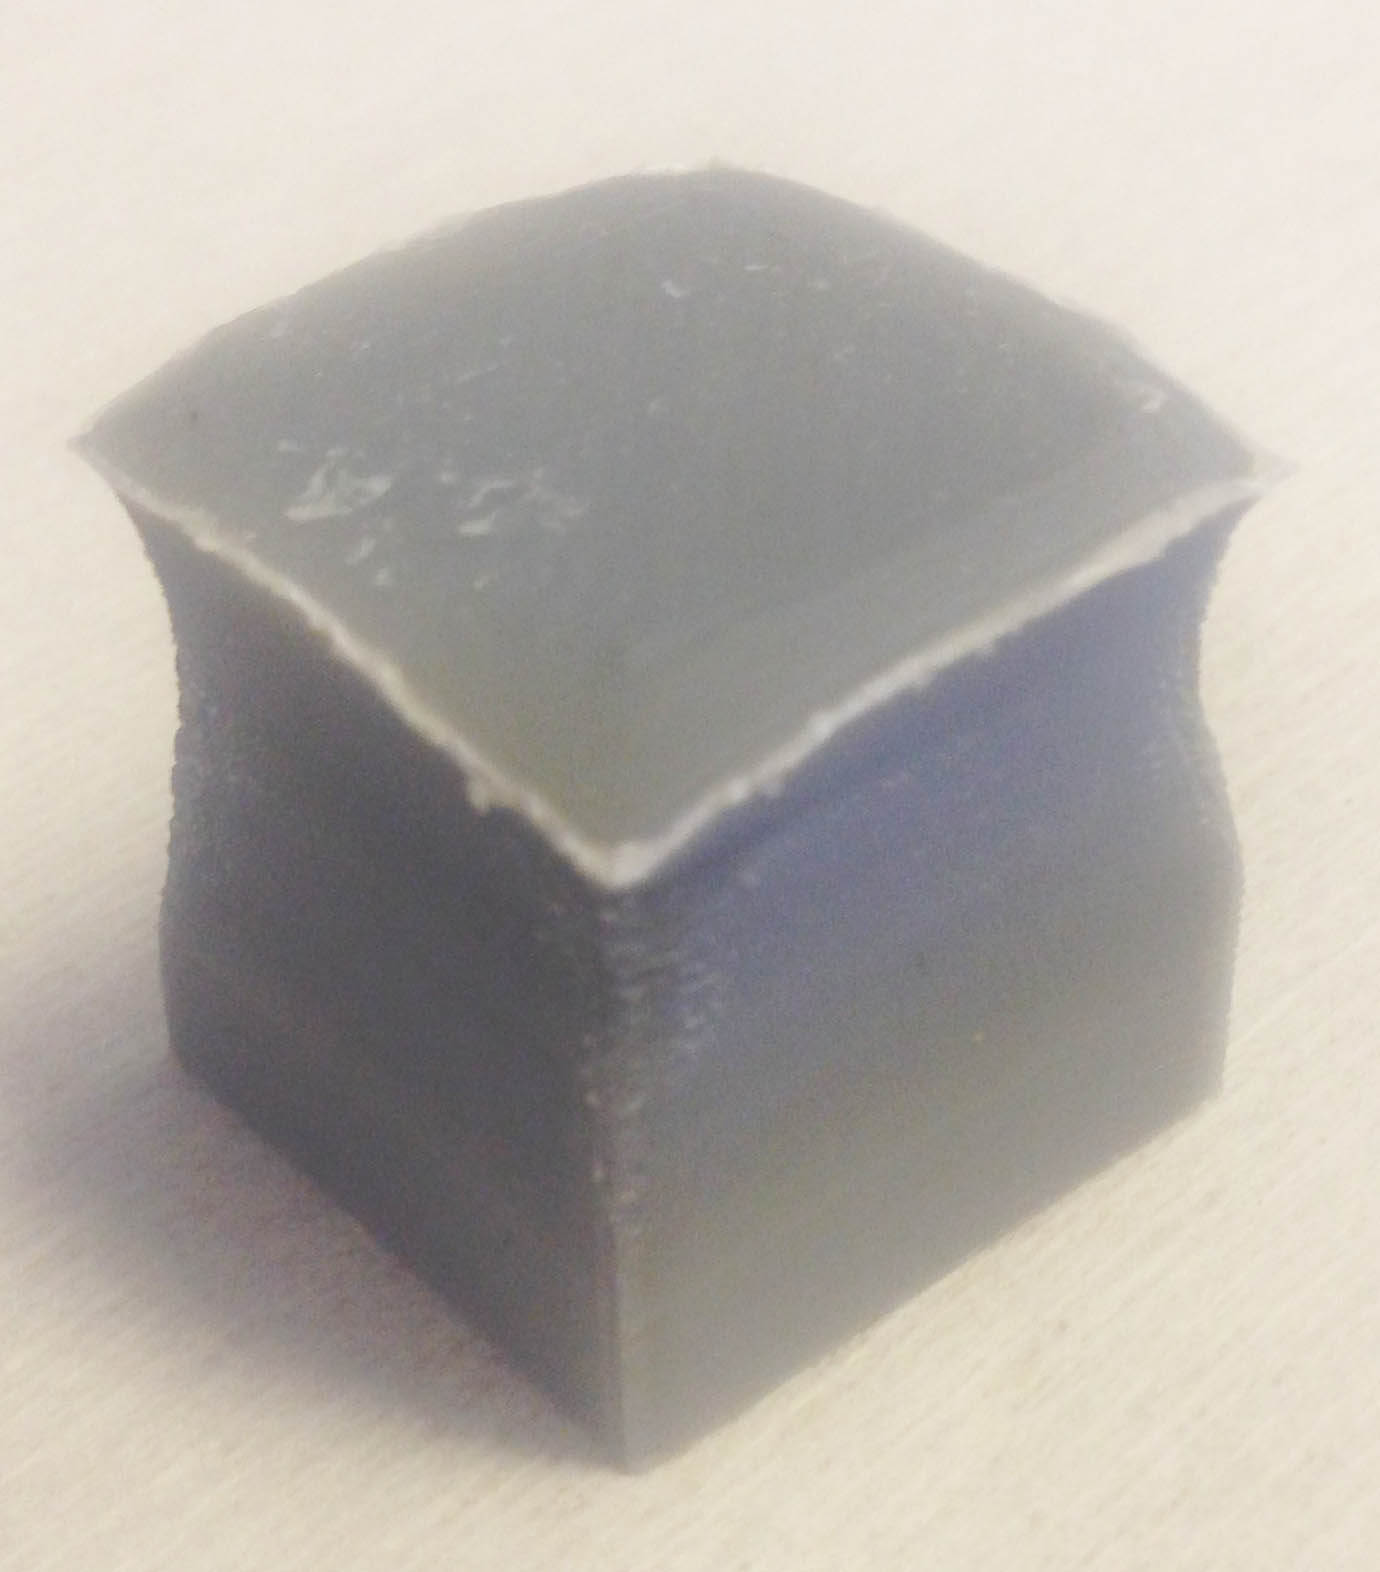
\includegraphics[height=4.6cm,width=4.6cm]{Figs5//1.JPG}
		\end{minipage}
        }
        \subfigure[]{
    \begin{minipage}[t]{0.35\textwidth}
			\centering
			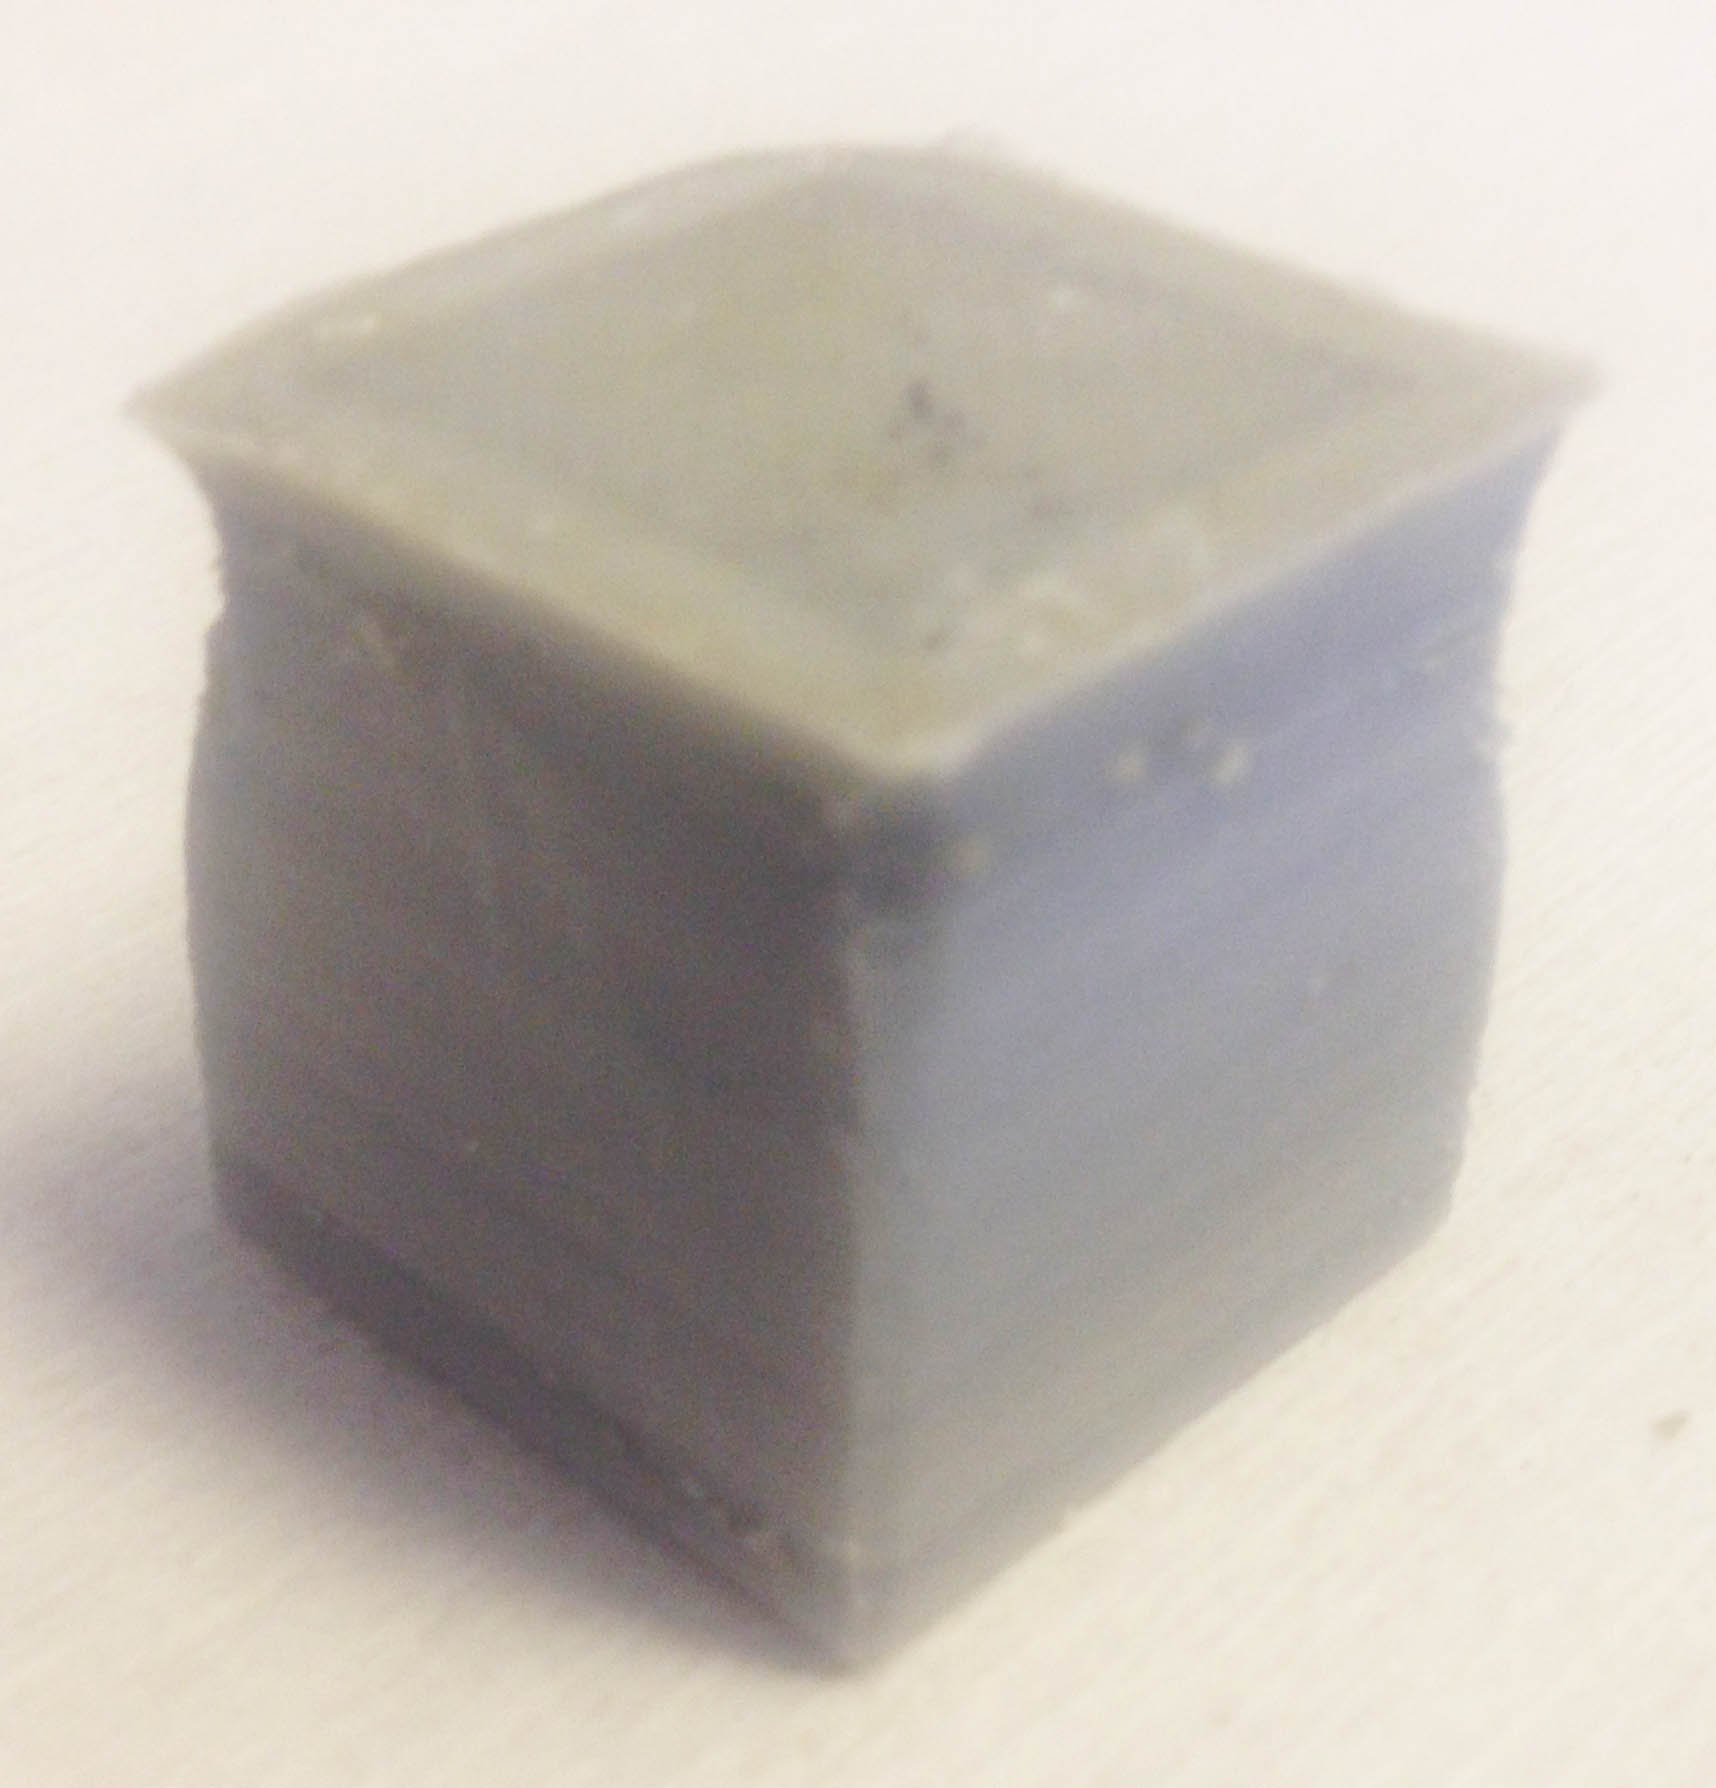
\includegraphics[height=4.6cm,width=4.6cm]{Figs5//2.JPG}
		\end{minipage}
	}
        \subfigure[]{
    \begin{minipage}[t]{0.35\textwidth}
			\centering
			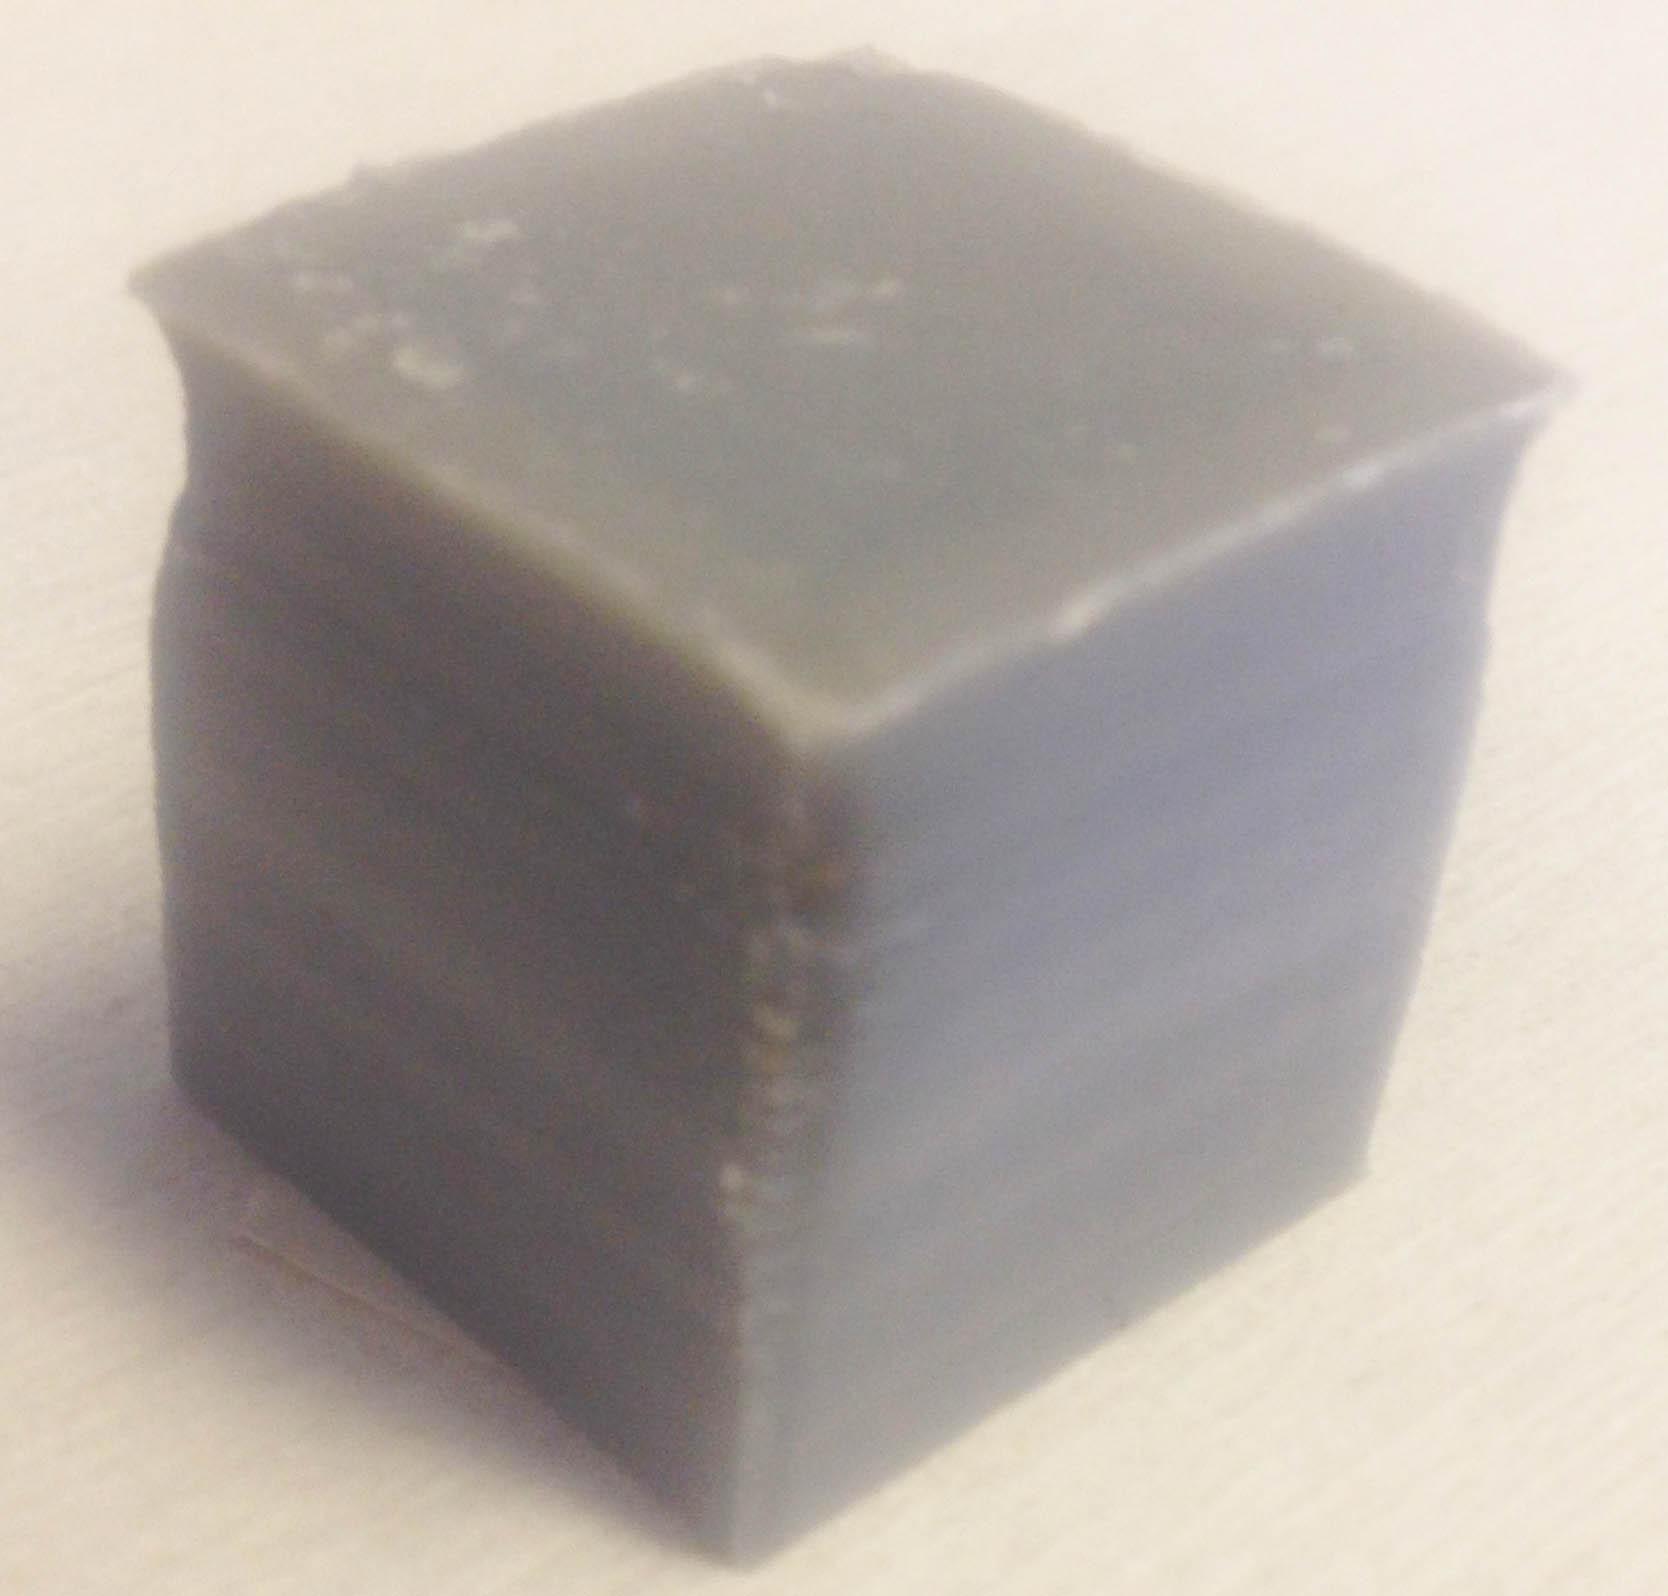
\includegraphics[height=4.6cm,width=4.6cm]{Figs5//3.JPG}
		\end{minipage}
	}
    \subfigure[]{
    \begin{minipage}[t]{0.35\textwidth}
			\centering
			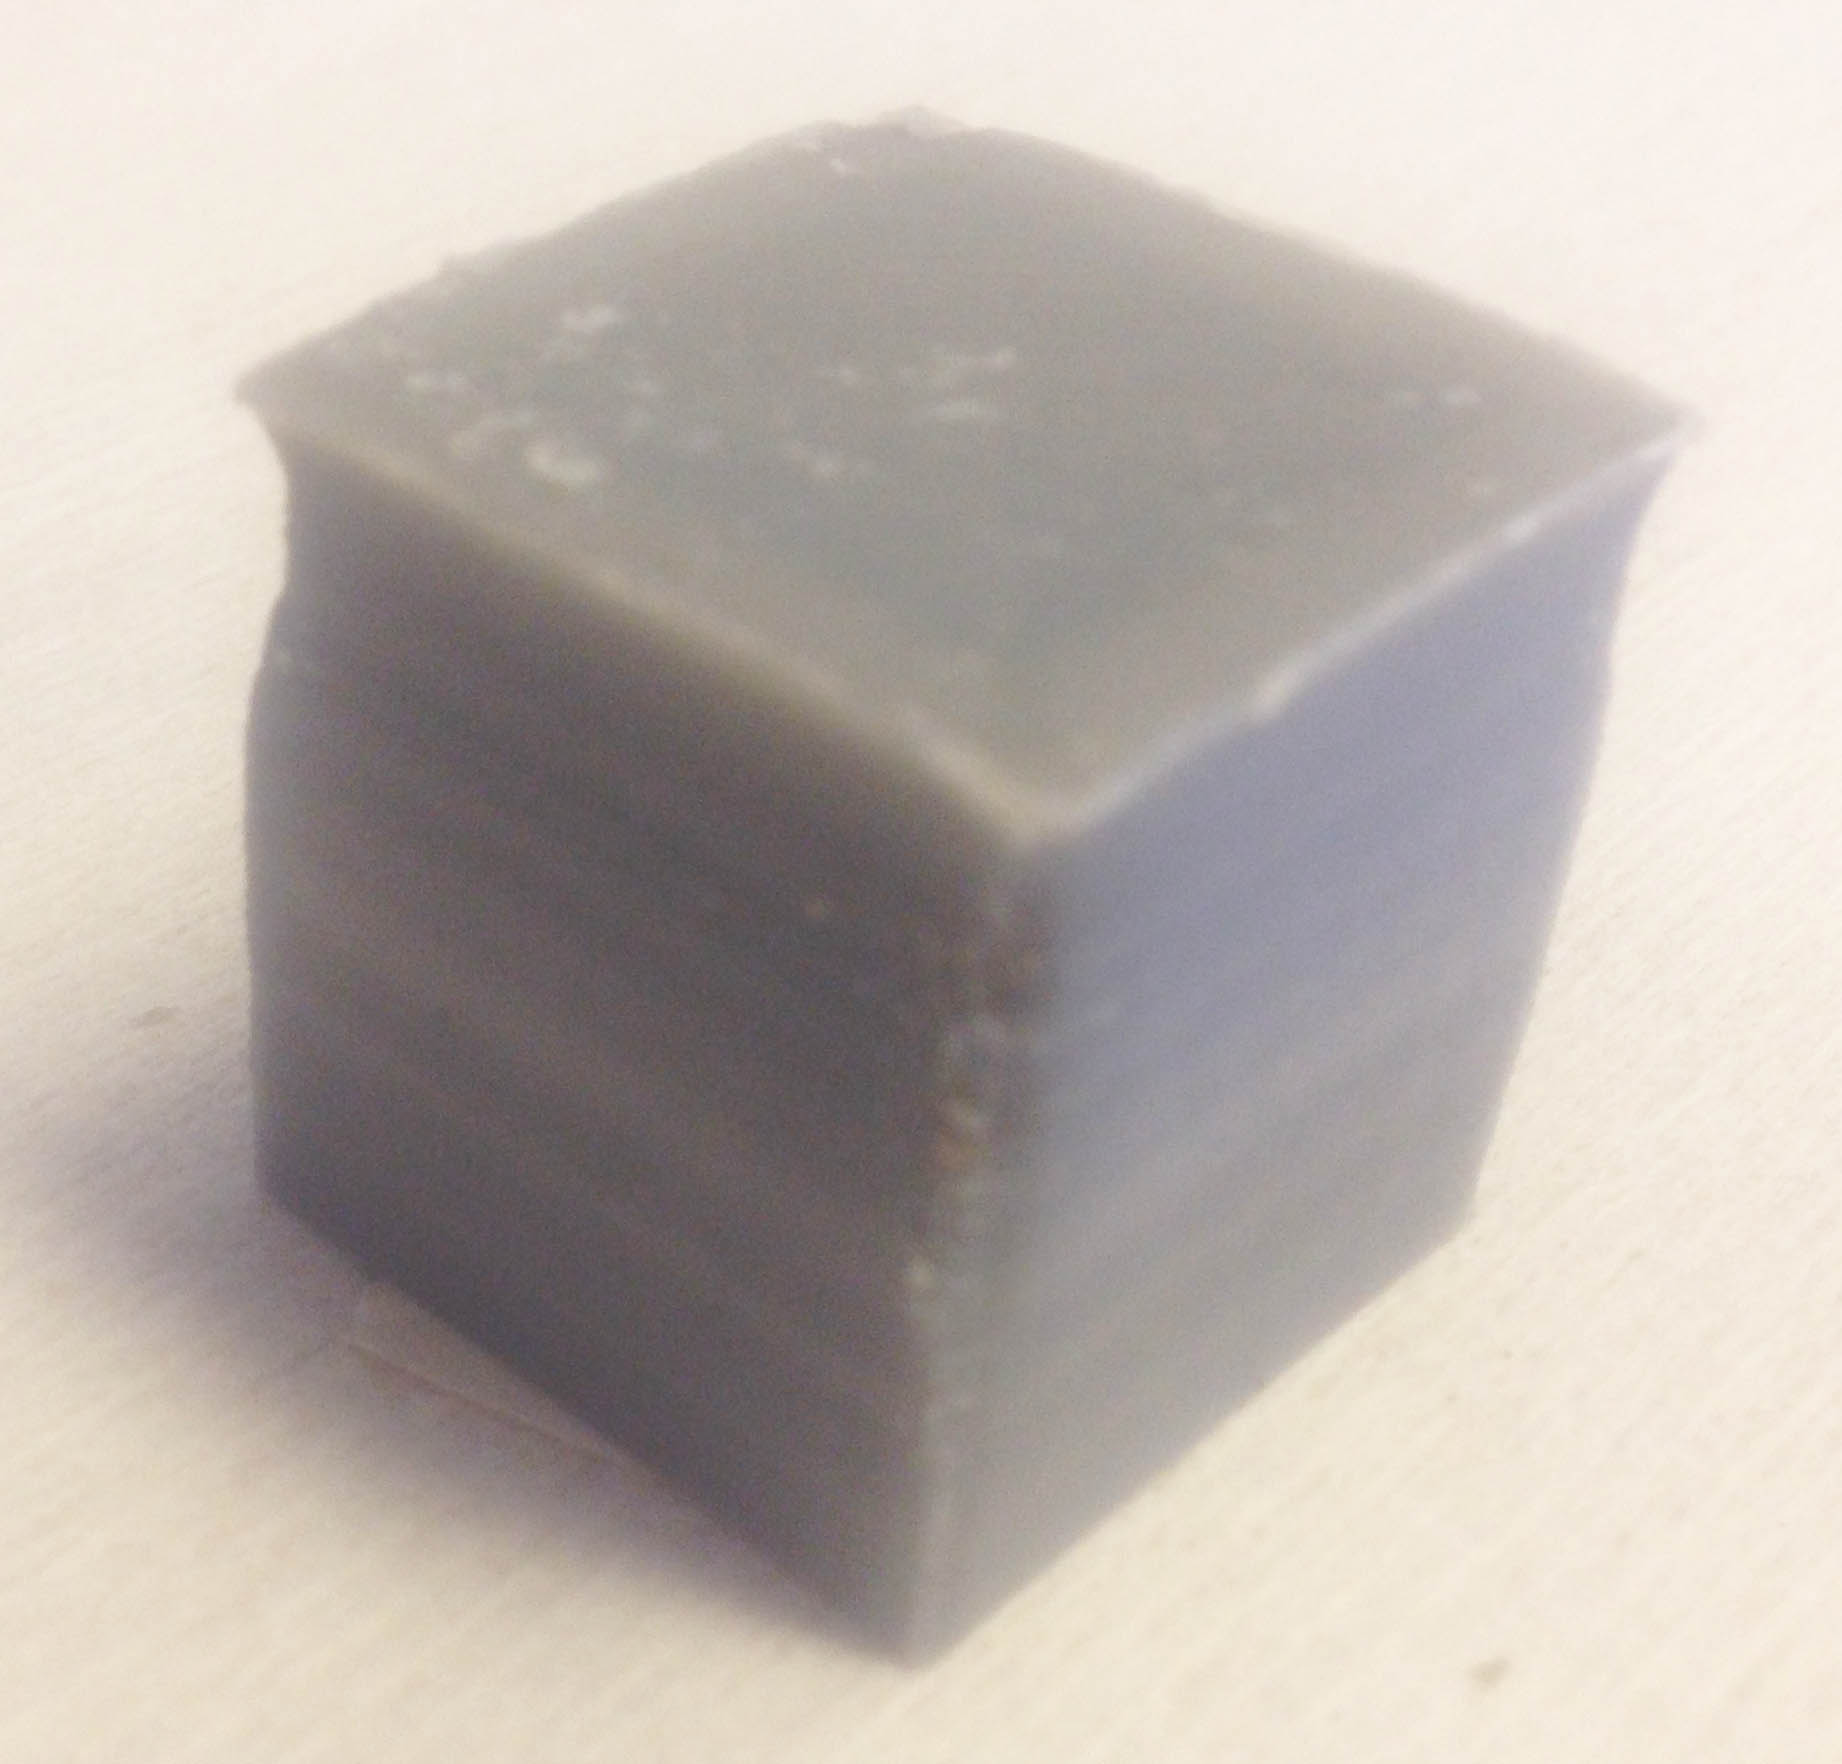
\includegraphics[height=4.6cm]{Figs5//4.JPG}
		\end{minipage}
	}
    \subfigure[]{
    \begin{minipage}[t]{0.35\textwidth}
			\centering
			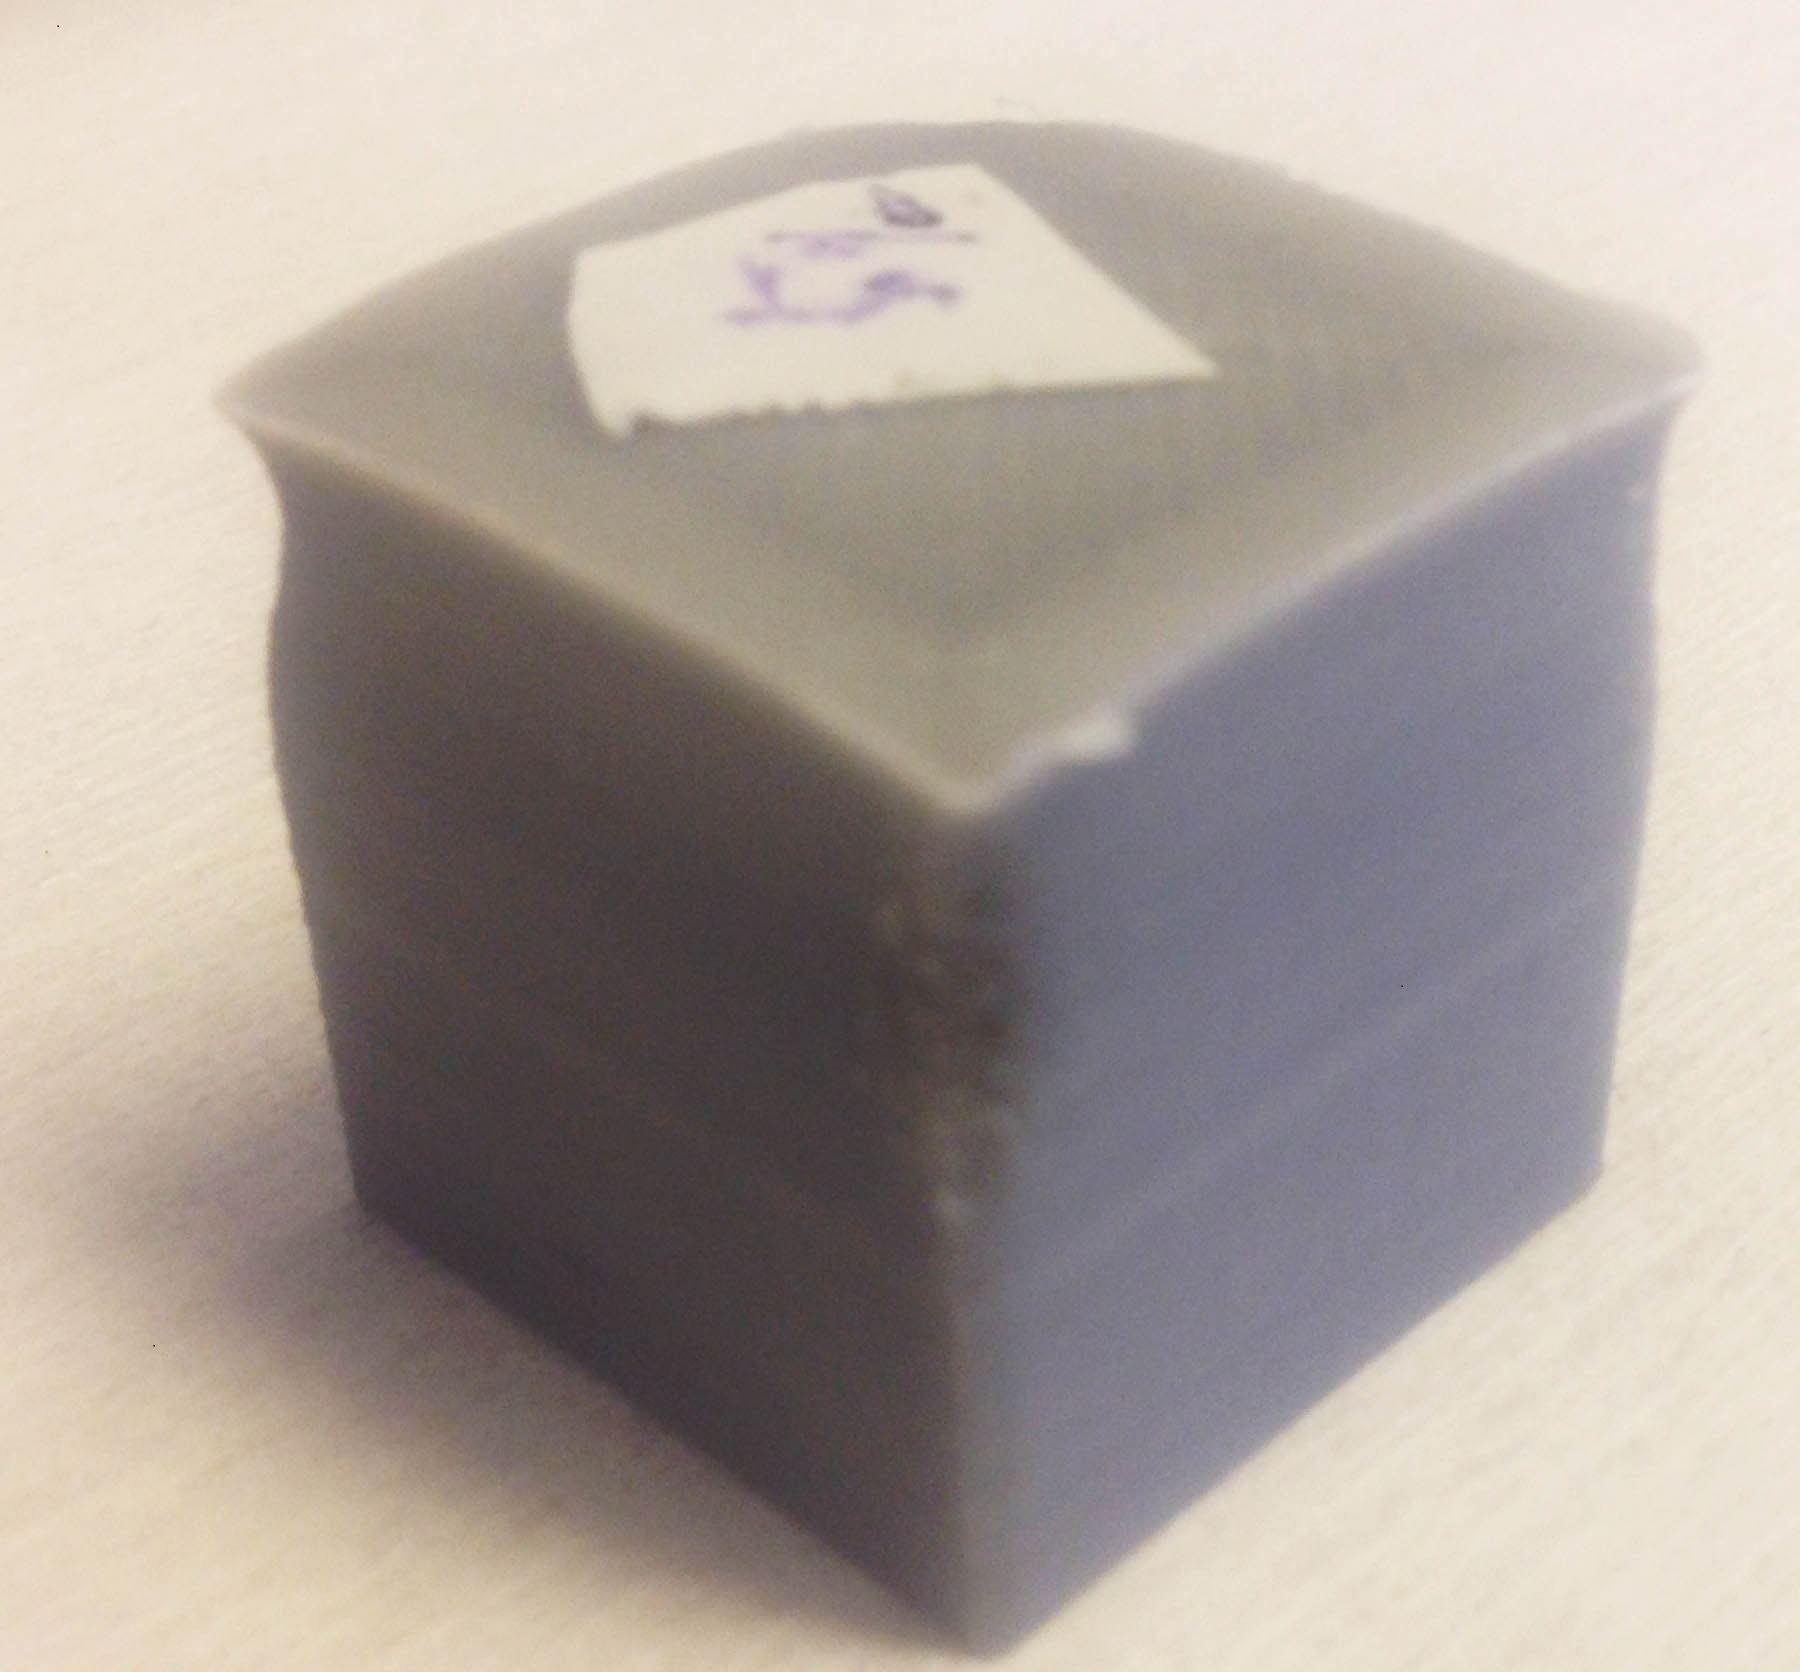
\includegraphics[height=4.6cm,width=4.6cm]{Figs5//5.jpg}
		\end{minipage}
	}
    \subfigure[]{
    \begin{minipage}[t]{0.35\textwidth}
			\centering
			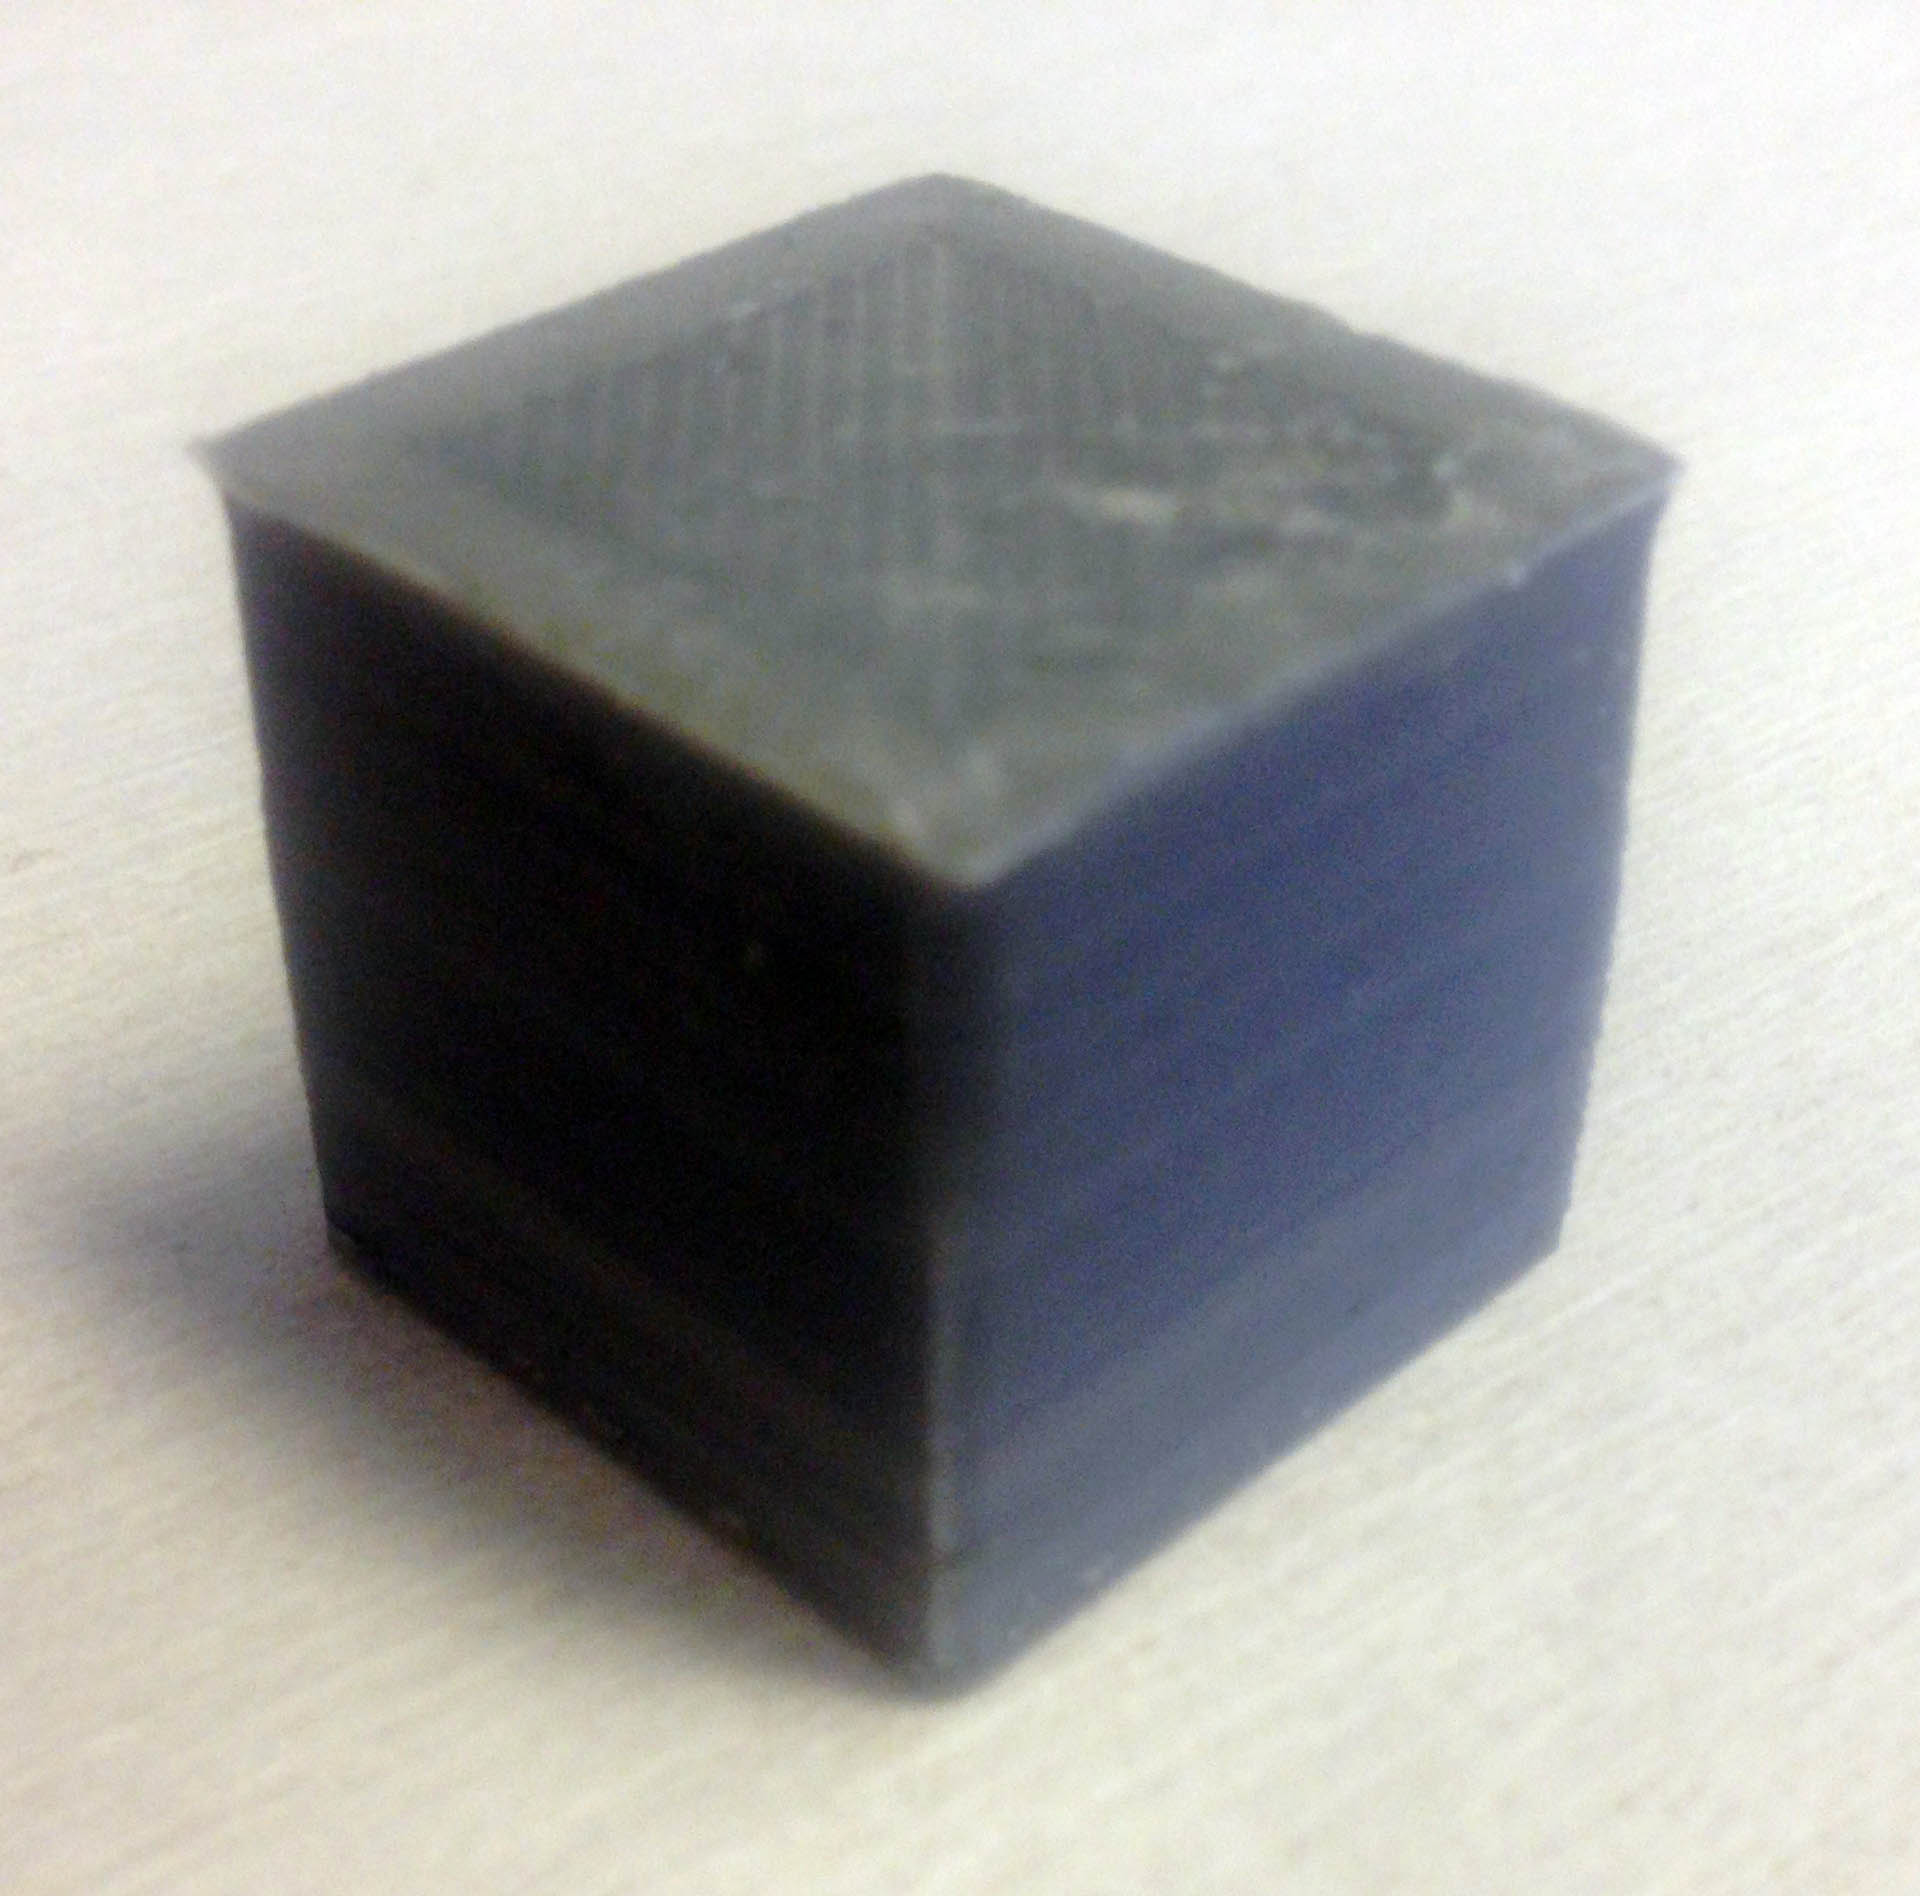
\includegraphics[height=4.6cm]{Figs5//6.JPG}
		\end{minipage}
	}
 
  \caption[The 3D-printed cubes]{\footnotesize The 3D-printed cubes made of(a)no pumice, (b)1 wt.$\%$ pumice, (c)2 wt.$\%$ pumice, (d)3 wt.$\%$ pumice, (e)4 wt.$\%$ pumice, (f)5 wt.$\%$ pumice, (g)6 wt.$\%$ pumice. }
  \label{Fig:cubes}
\end{figure}
\begin{figure}[htbp] % make the image in the middle of paragraph
	\centering
	\subfigure[]{
    \begin{minipage}[t]{0.2\textwidth}
			\centering
			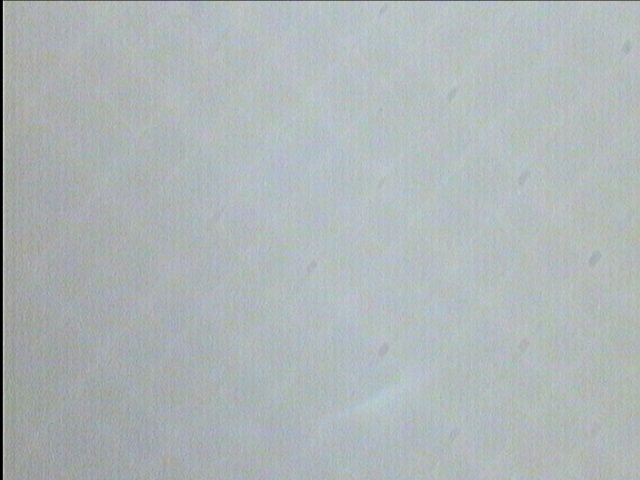
\includegraphics[height=2.5cm]{Figs5//block0.jpg}
		\end{minipage}
	}
    \subfigure[]{
    \begin{minipage}[t]{0.2\textwidth}
			\centering
			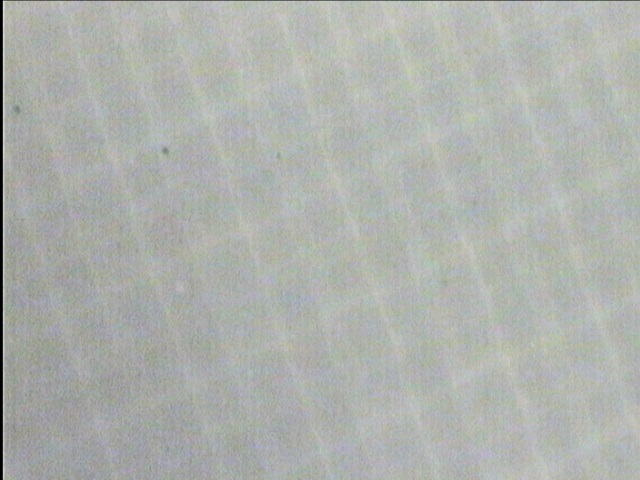
\includegraphics[height=2.5cm]{Figs5//block1.jpg}
		\end{minipage}
	}
    \subfigure[]{
    \begin{minipage}[t]{0.2\textwidth}
			\centering
			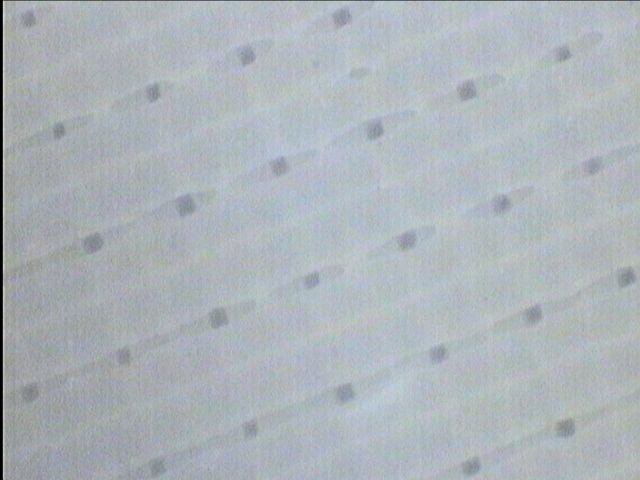
\includegraphics[height=2.5cm]{Figs5//block2.jpg}
		\end{minipage}
	}
    \subfigure[]{
    \begin{minipage}[t]{0.2\textwidth}
			\centering
			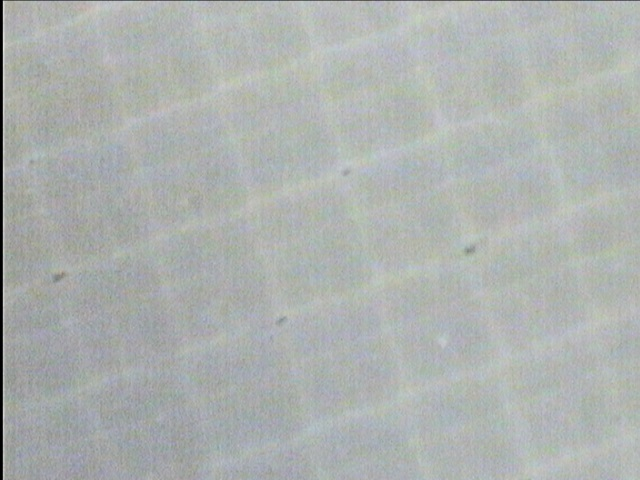
\includegraphics[height=2.5cm]{Figs5//block3.jpg}
		\end{minipage}
	}
  \subfigure[]{
    \begin{minipage}[t]{0.2\textwidth}
			\centering
			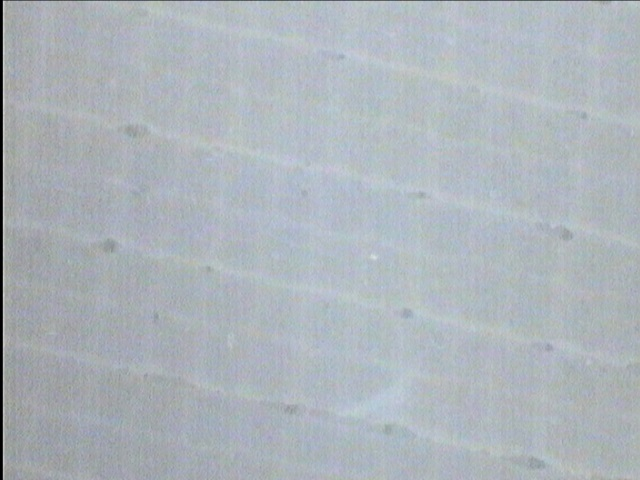
\includegraphics[height=2.5cm]{Figs5//block4.jpg}
		\end{minipage}
	}
     \subfigure[]{
    \begin{minipage}[t]{0.2\textwidth}
			\centering
			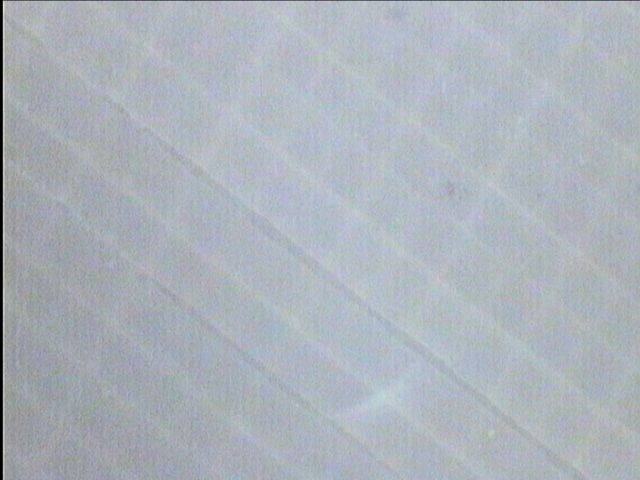
\includegraphics[height=2.5cm]{Figs5//block5.jpg}
		\end{minipage}
	}
     \subfigure[]{
    \begin{minipage}[t]{0.2\textwidth}
			\centering
			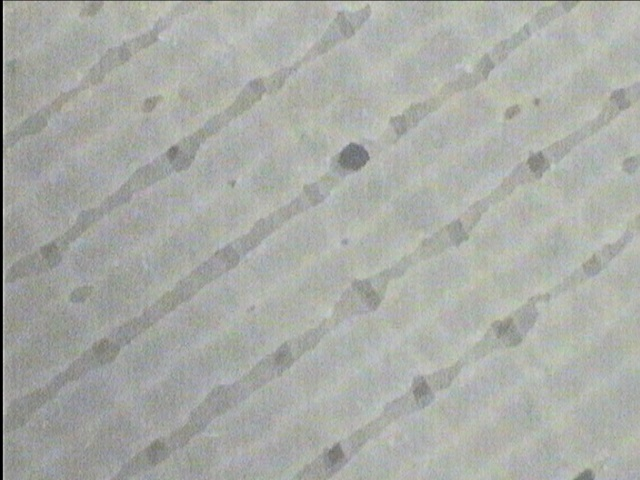
\includegraphics[height=2.5cm]{Figs5//block6.jpg}
		\end{minipage}
	}
  \caption[The infill lines on the cubes]{\footnotesize The infill lines on the cubes made with (a)no pumice, (b)1 wt.$\%$ pumice, (c)2 wt.$\%$ pumice, (d)3 wt.$\%$ pumice, (e)4 wt.$\%$ pumice, (f)5 wt.$\%$ pumice, (g)6 wt.$\%$ pumice.}
  \label{Fig:cube layer}
\end{figure}
\begin{figure}[htbp] % make the image in the middle of paragraph
	\centering
	\subfigure[]{
    \begin{minipage}[t]{0.2\textwidth}
			\centering
			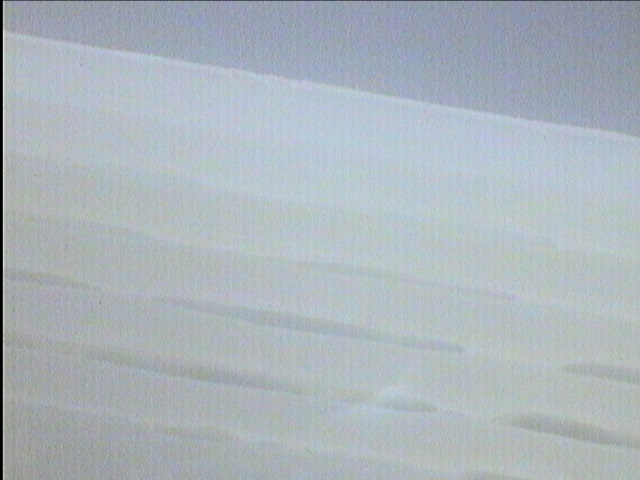
\includegraphics[height=2.5cm]{Figs5//cblock0.jpg}
		\end{minipage}
	}
    \subfigure[]{
    \begin{minipage}[t]{0.2\textwidth}
			\centering
			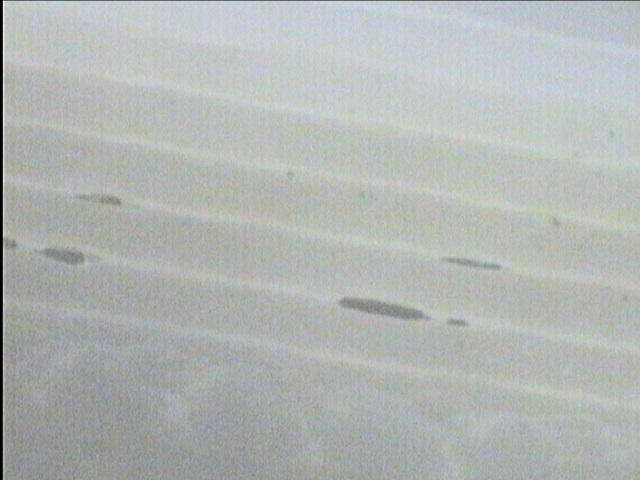
\includegraphics[height=2.5cm]{Figs5//cblock1.jpg}
		\end{minipage}
	}
    \subfigure[]{
    \begin{minipage}[t]{0.2\textwidth}
			\centering
			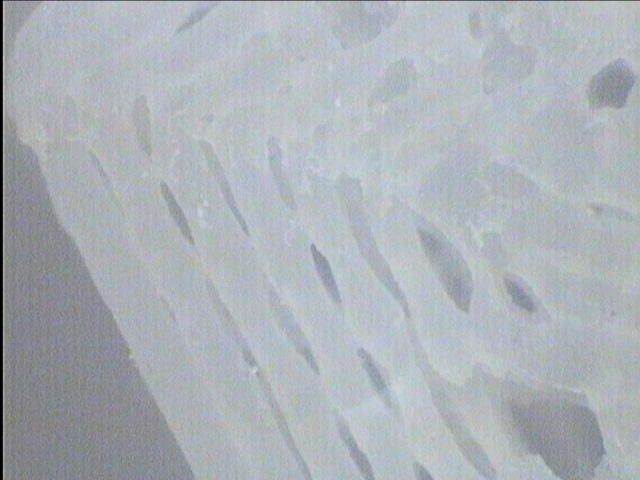
\includegraphics[height=2.5cm]{Figs5//cblock2.jpg}
		\end{minipage}
	}
    \subfigure[]{
    \begin{minipage}[t]{0.2\textwidth}
			\centering
			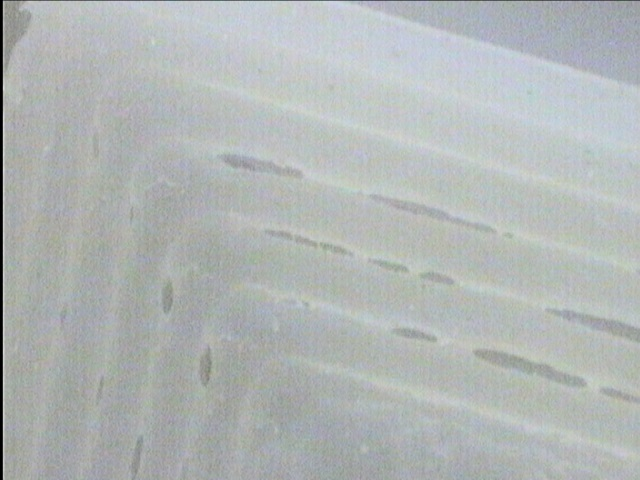
\includegraphics[height=2.5cm]{Figs5//cblock3.jpg}
		\end{minipage}
	}
  \subfigure[]{
    \begin{minipage}[t]{0.2\textwidth}
			\centering
			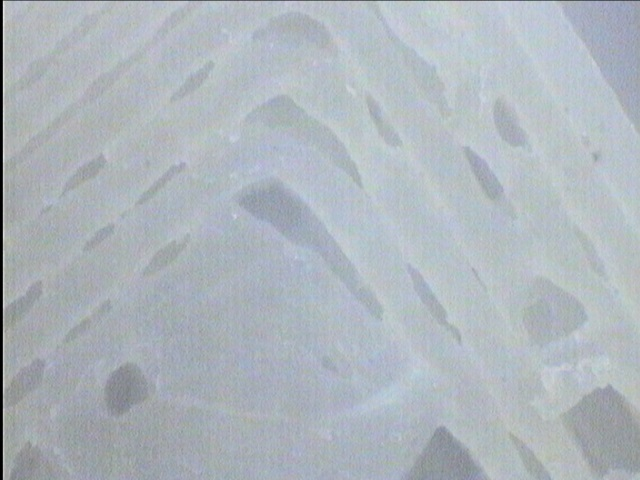
\includegraphics[height=2.5cm]{Figs5//cblock4.jpg}
		\end{minipage}
	}
     \subfigure[]{
    \begin{minipage}[t]{0.2\textwidth}
			\centering
			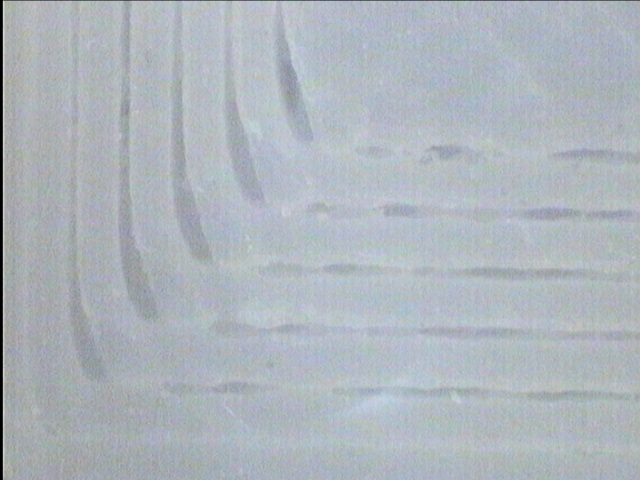
\includegraphics[height=2.5cm]{Figs5//cblock5.jpg}
		\end{minipage}
	}
     \subfigure[]{
    \begin{minipage}[t]{0.2\textwidth}
			\centering
			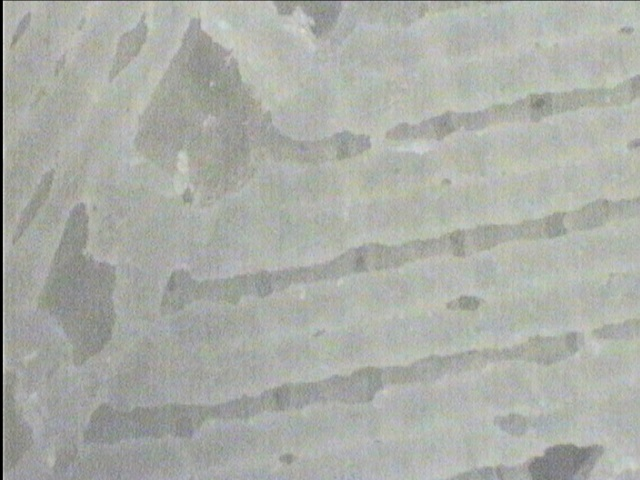
\includegraphics[height=2.5cm]{Figs5//cblock6.jpg}
		\end{minipage}
	}
  \caption[The wall lines on the cubes]{\footnotesize The wall lines on the cubes made of (a)no pumice, (b)1 wt.$\%$ pumice, (c)2 wt.$\%$ pumice, (d)3 wt.$\%$ pumice, (e)4 wt.$\%$ pumice, (f)5 wt.$\%$ pumice, (g)6 wt.$\%$ pumice. }
  \label{Fig:cube layer2}
\end{figure}
As Figure \ref{Fig:cube layer} and \ref{Fig:cube layer2} shows, the details of the cubes are different which are captured by the microscope and connected camera. The one made by pure ABS has almost no gaps between lines but it warps seriously. Considering the geometrical accuracy and the gaps between lays and lines, the best one is made by 5 wt.\% pumice. Checking their corresponding filament, the big gaps between lines are stem from the diameter which is larger than 3.00mm or smaller than 2.80mm. The UM2 is quite sensitive to the size of the filament. And the pumice powder decreases the level of warp according to the geometrical accuracy of the cubes. 

\begin{itemize}
\item Waveguides
\end{itemize}
The printing of waveguides is the most time-consuming work in this project. The challenge is derived from the materials we utilised are really new. The printability of them is uncertain. The most printable filament is fabricated with 2 wt.$\%$ pumice and ABS and has 2.85-3.05mm diameter. It cannot be denied that filament consistency also influenced the printability of it but the guess work could demonstrate whether it is printable. As for the practical usage of the waveguides, the flatness of inner wall contributes a lot. Therefore, it is essential to compare the performance of their inner wall. 

\begin{figure}[htbp] % make the image in the middle of paragraph
	\centering
	\subfigure[]{
    \begin{minipage}[t]{0.35\textwidth}
			\centering
			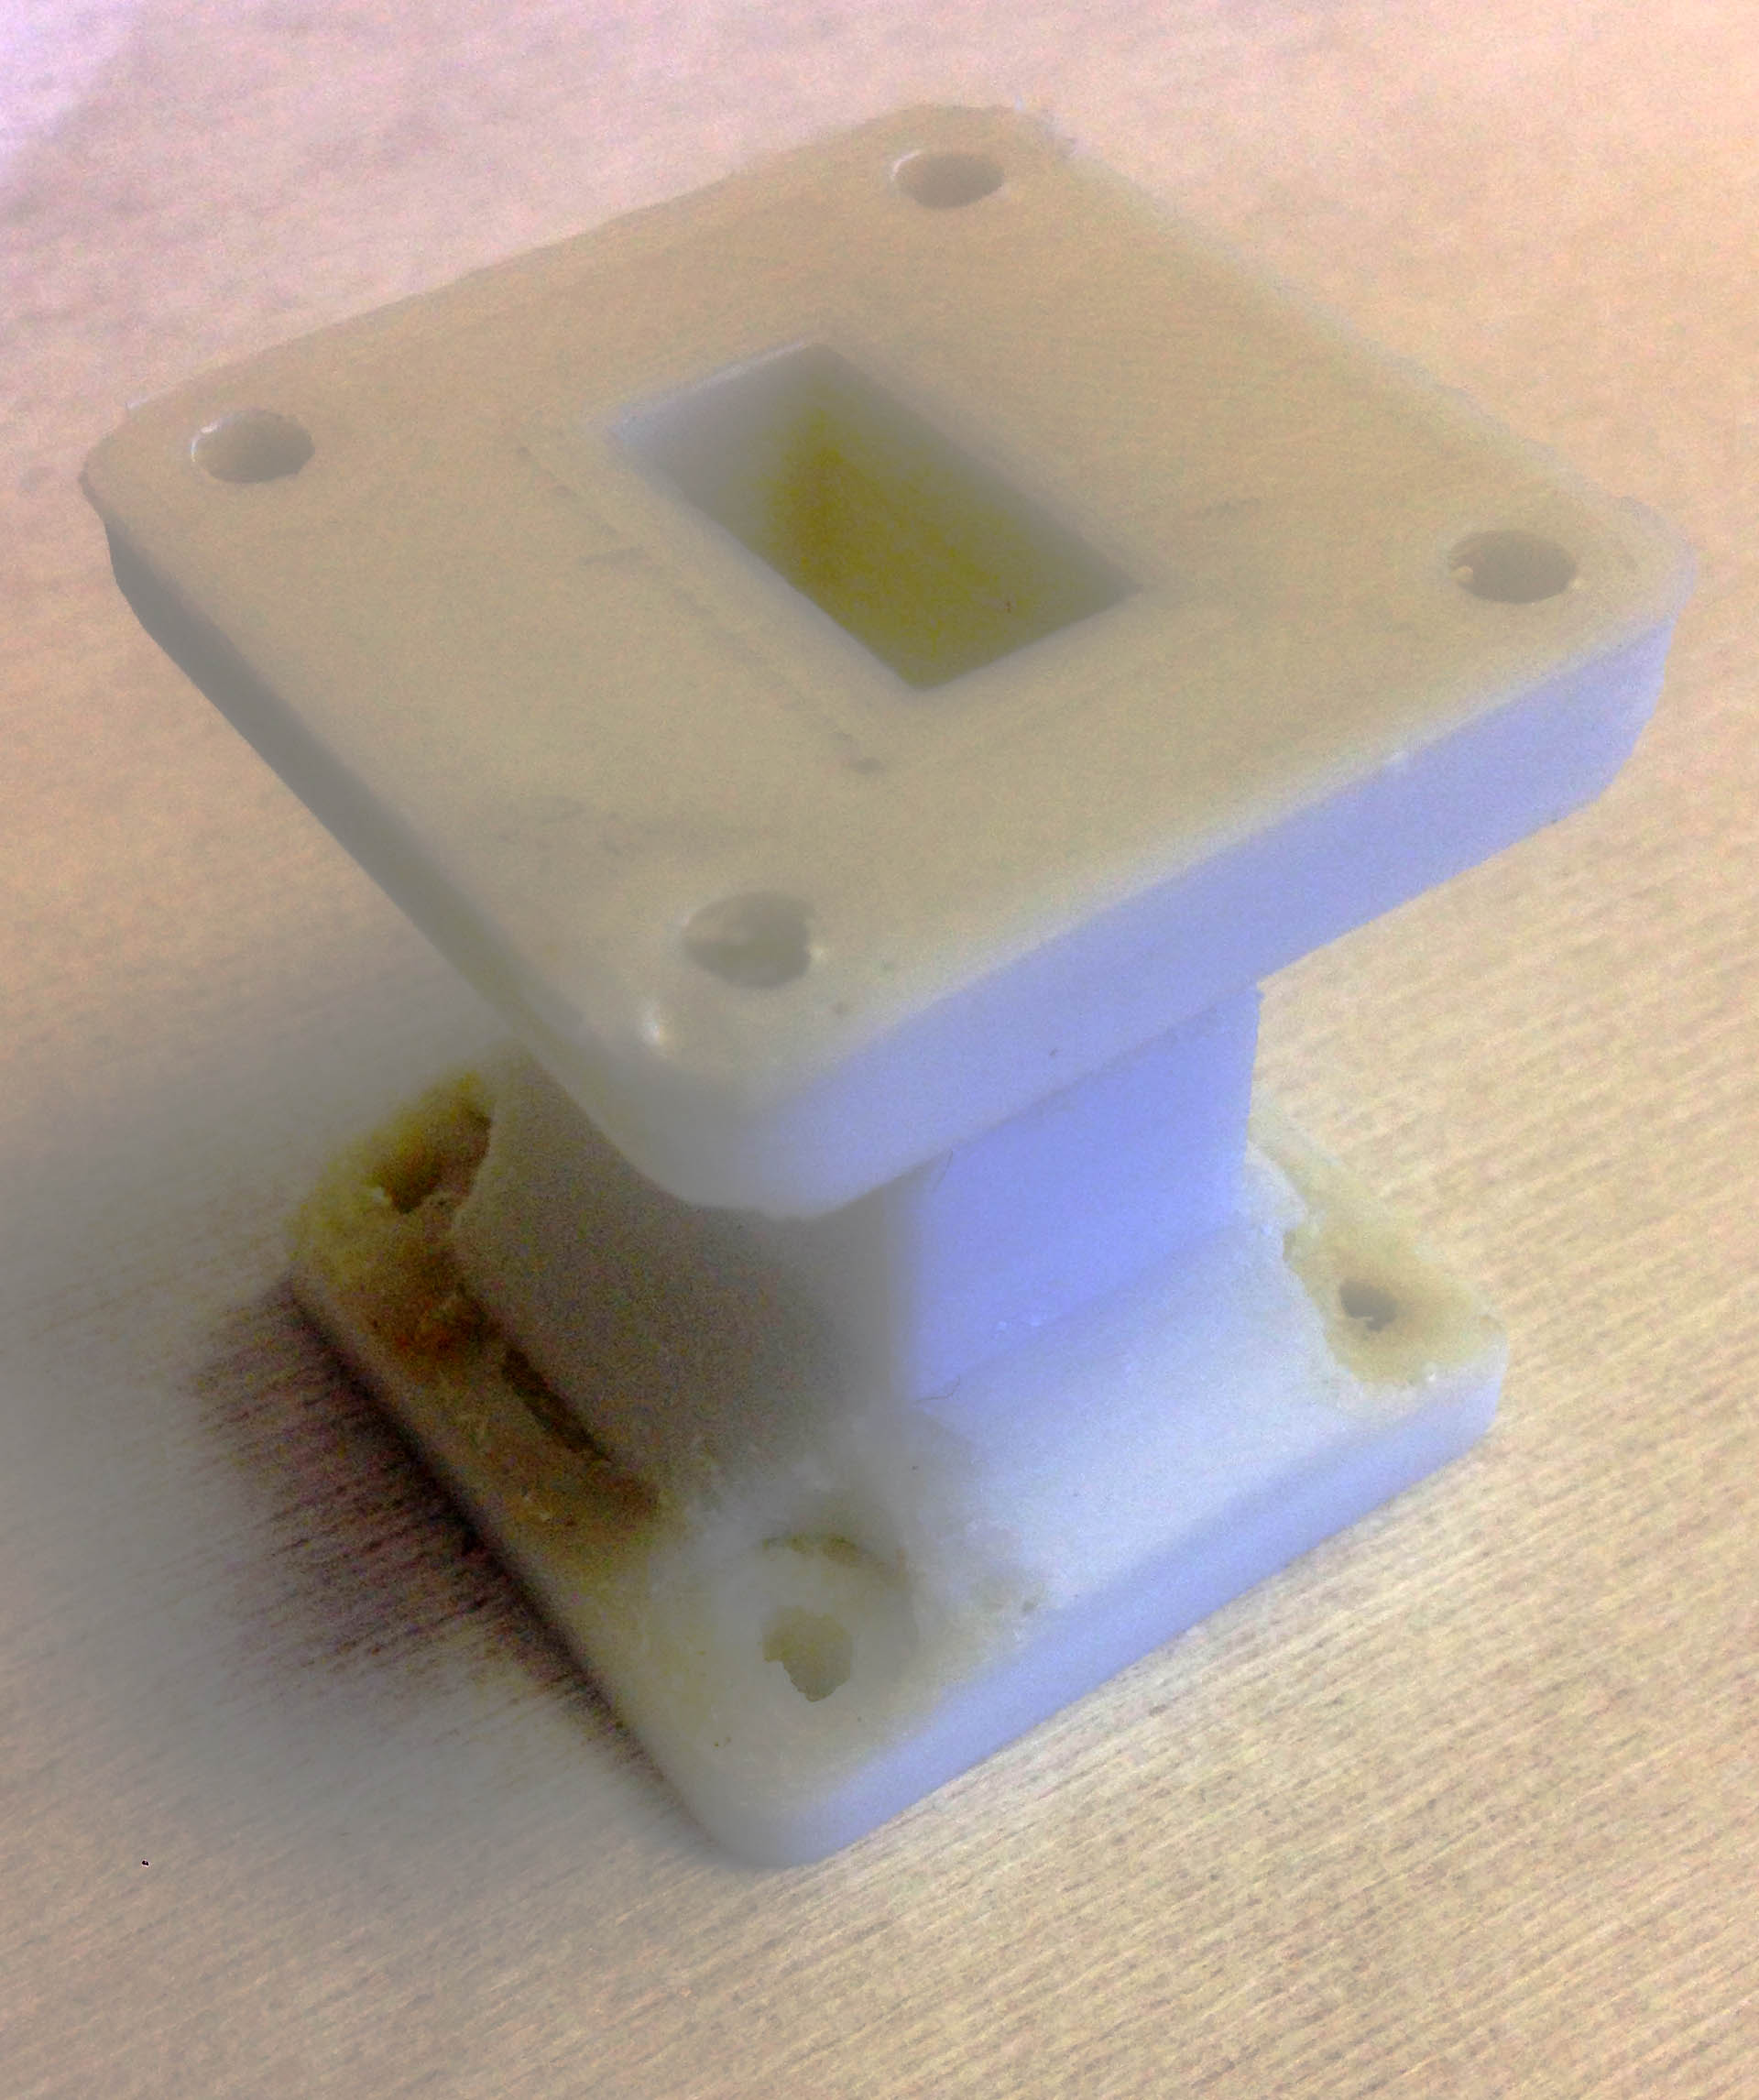
\includegraphics[height=5cm]{Figs5//0_pumice.JPG}
		\end{minipage}
	}
	\subfigure[]{
		\begin{minipage}[t]{0.35\textwidth}
			\centering
			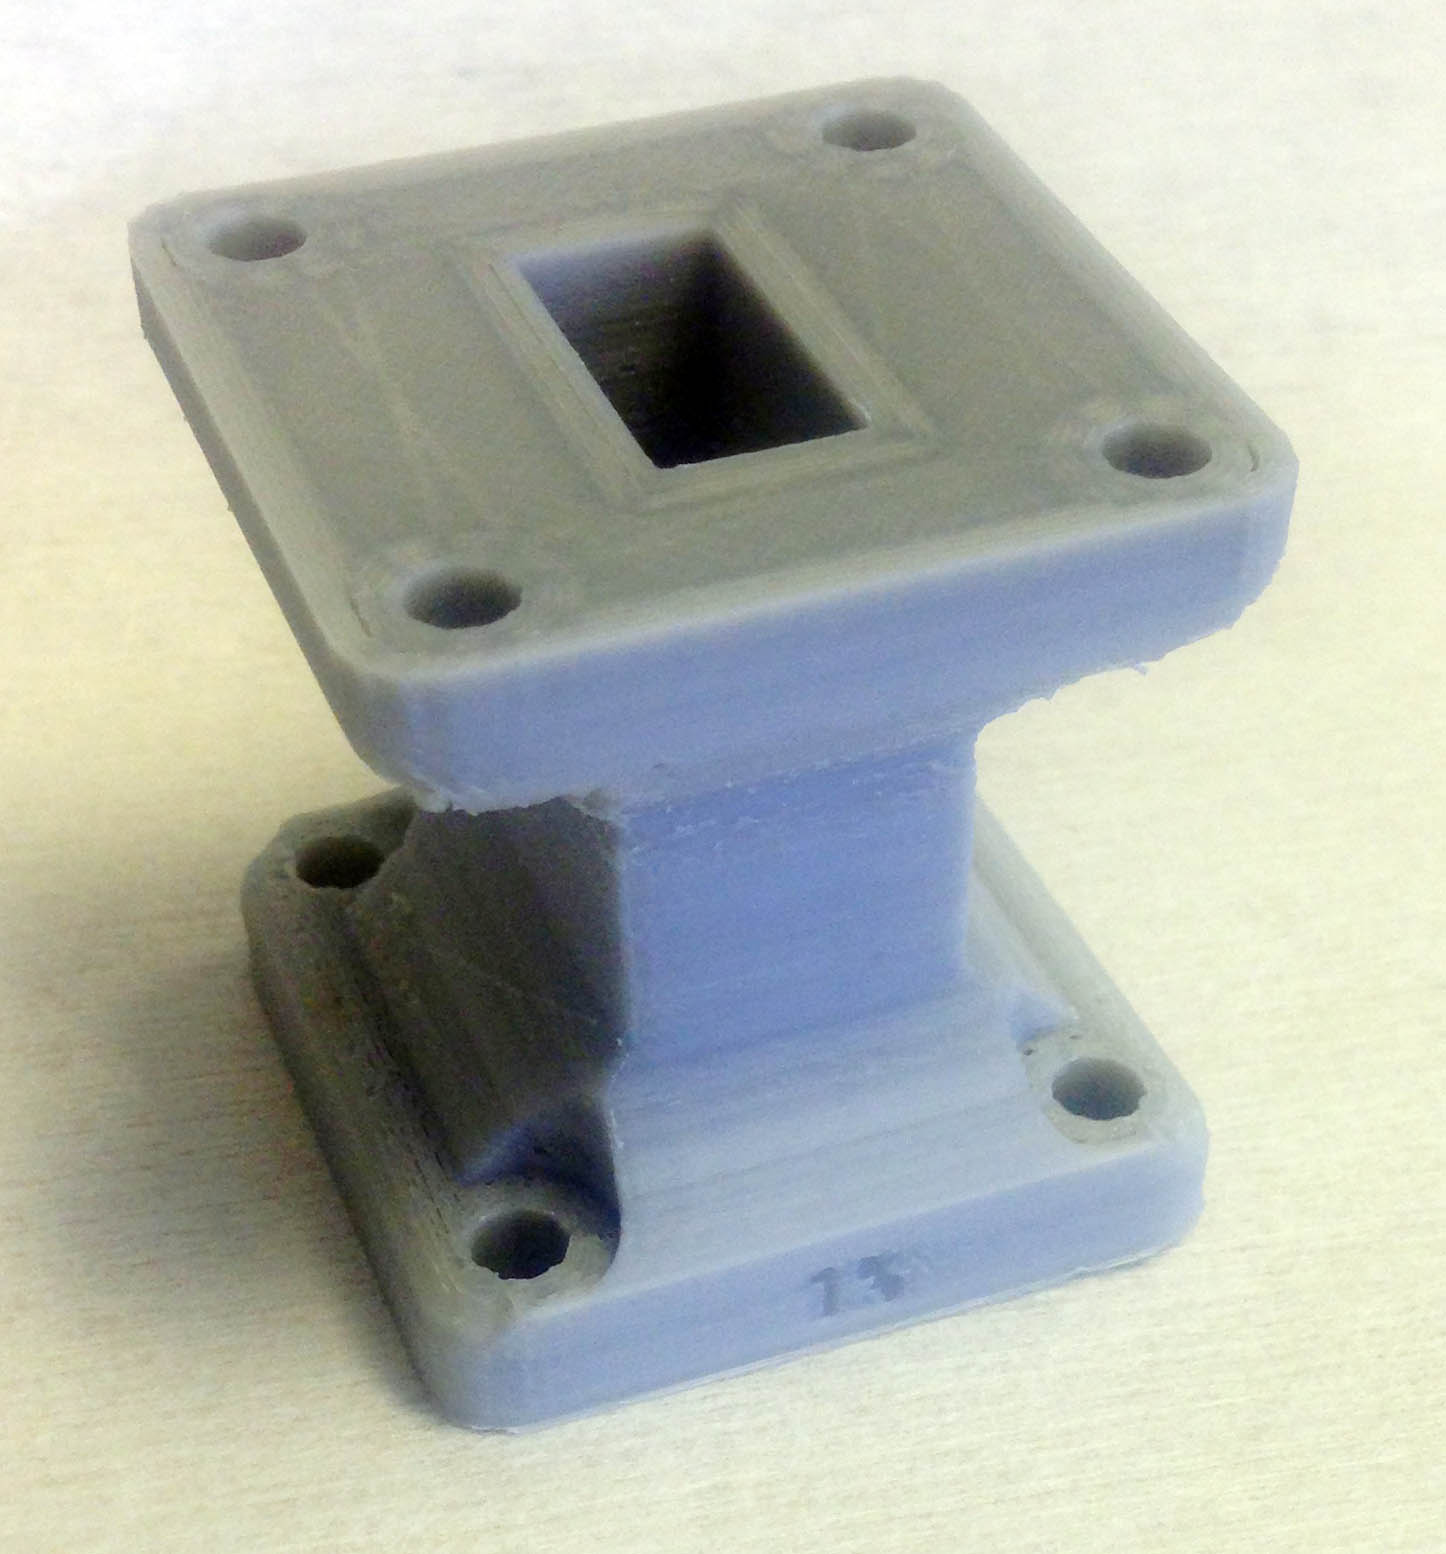
\includegraphics[height=5cm]{Figs5//1_pumice.JPG}
		\end{minipage}
        }
        \subfigure[]{
    \begin{minipage}[t]{0.35\textwidth}
			\centering
			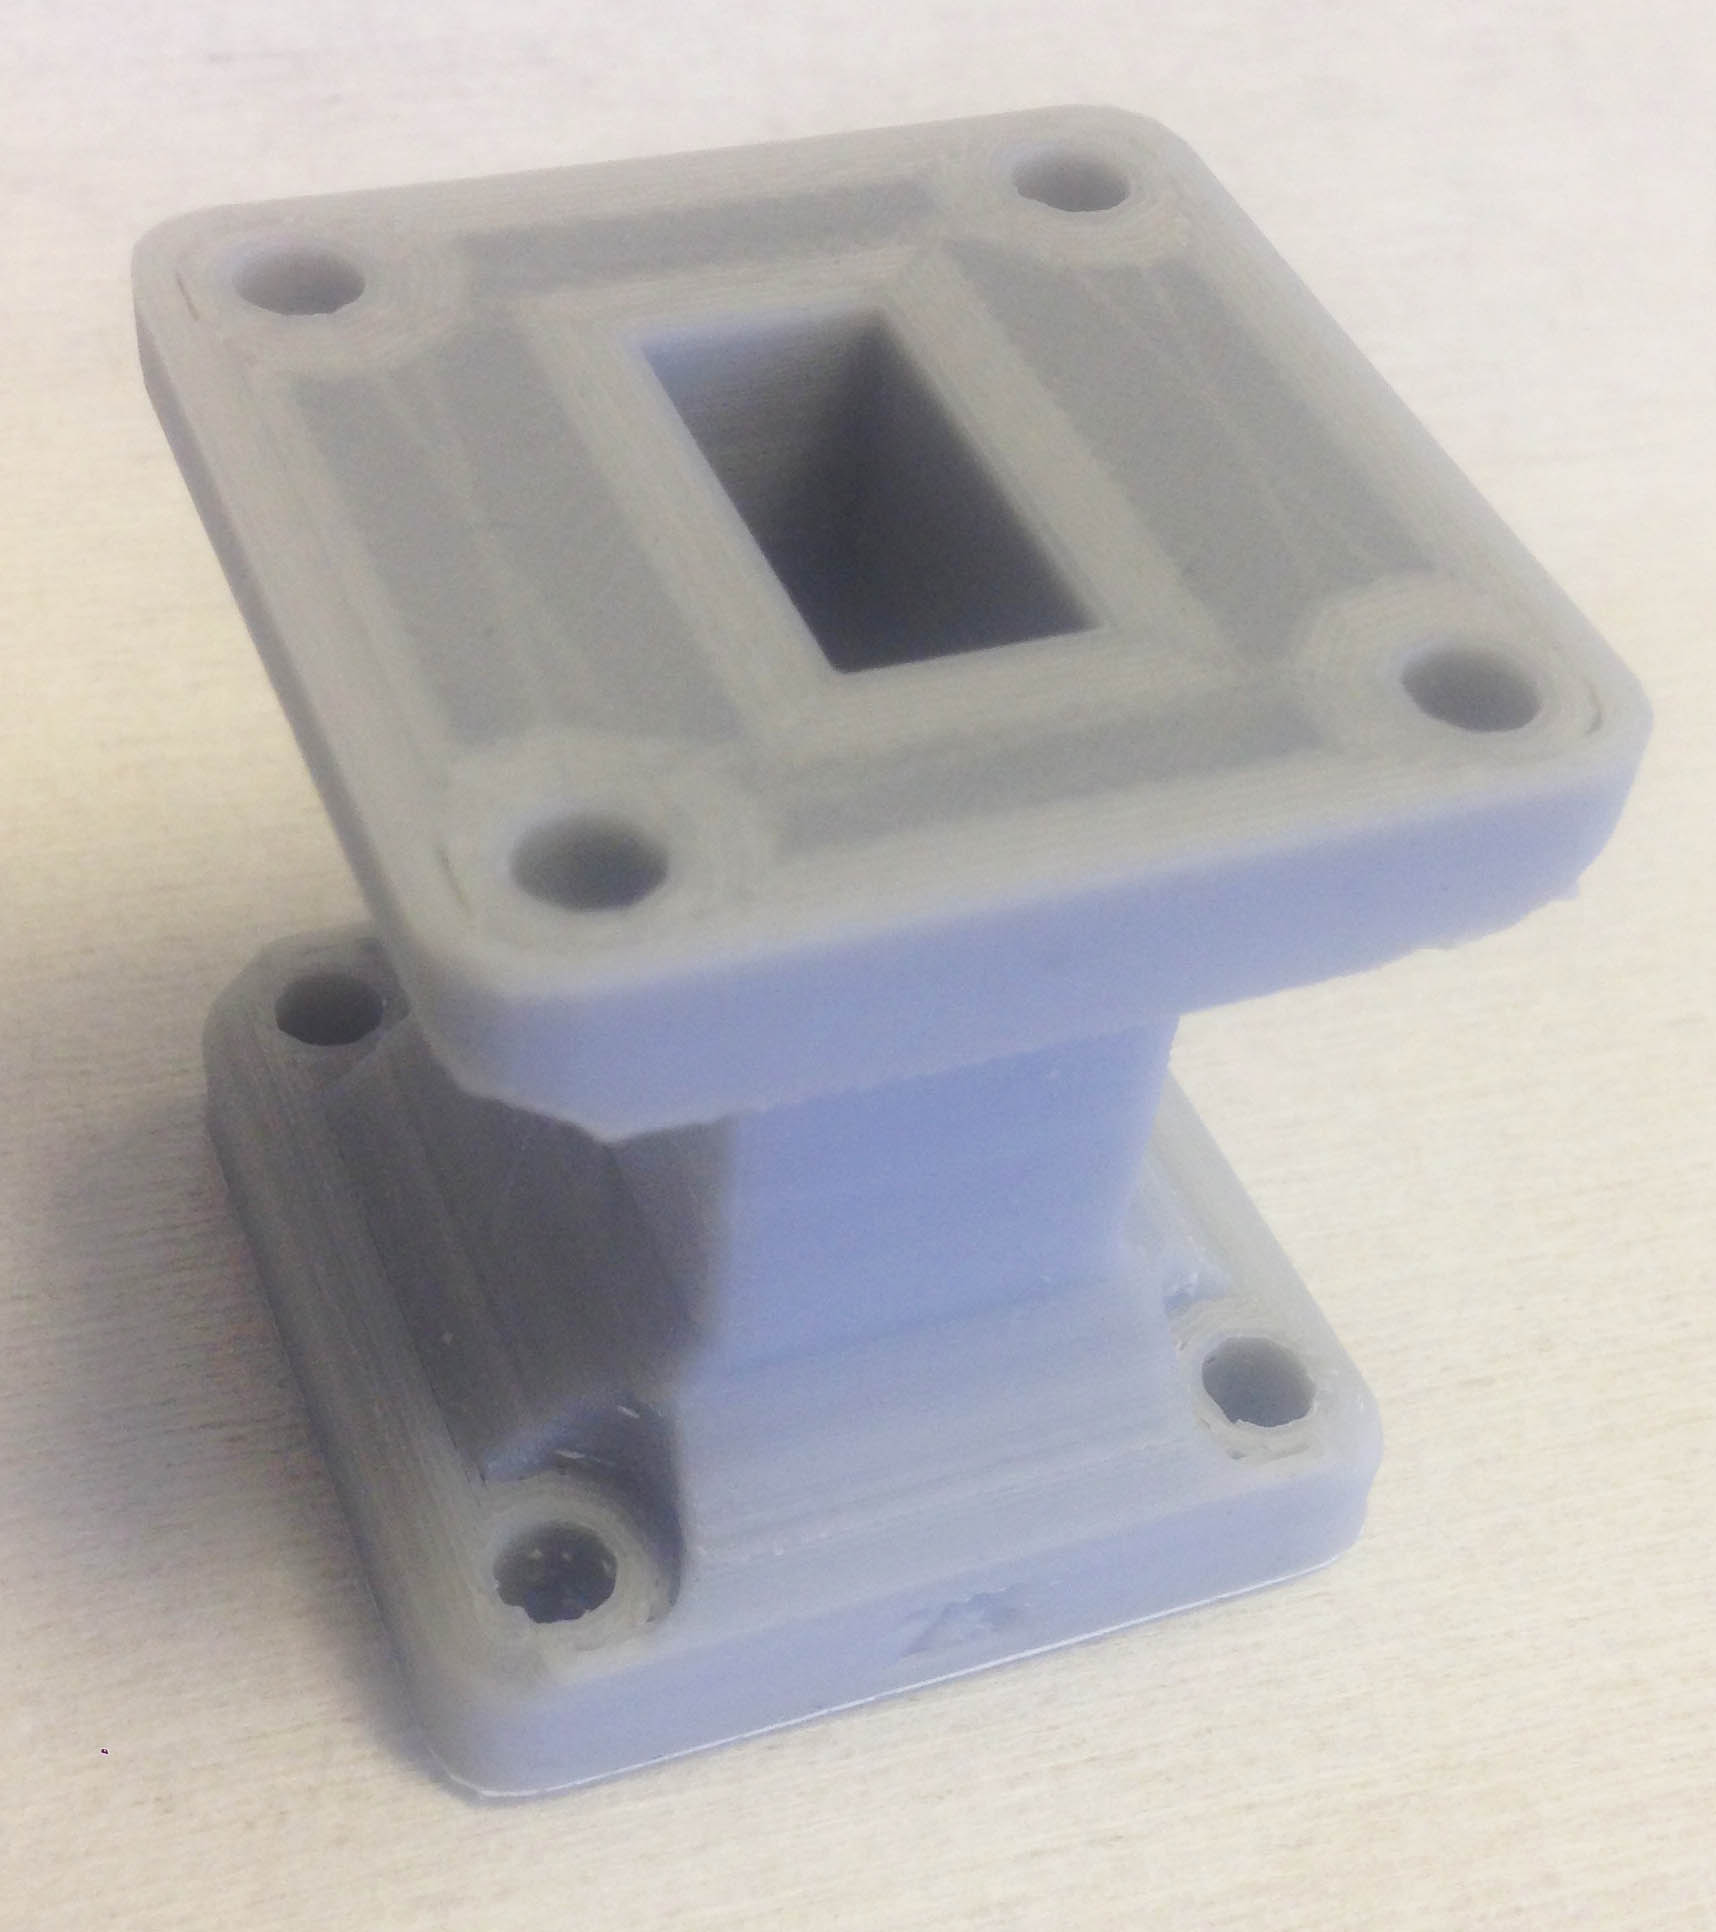
\includegraphics[height=5cm]{Figs5//2_pumice.JPG}
		\end{minipage}
	}
        \subfigure[]{
    \begin{minipage}[t]{0.35\textwidth}
			\centering
			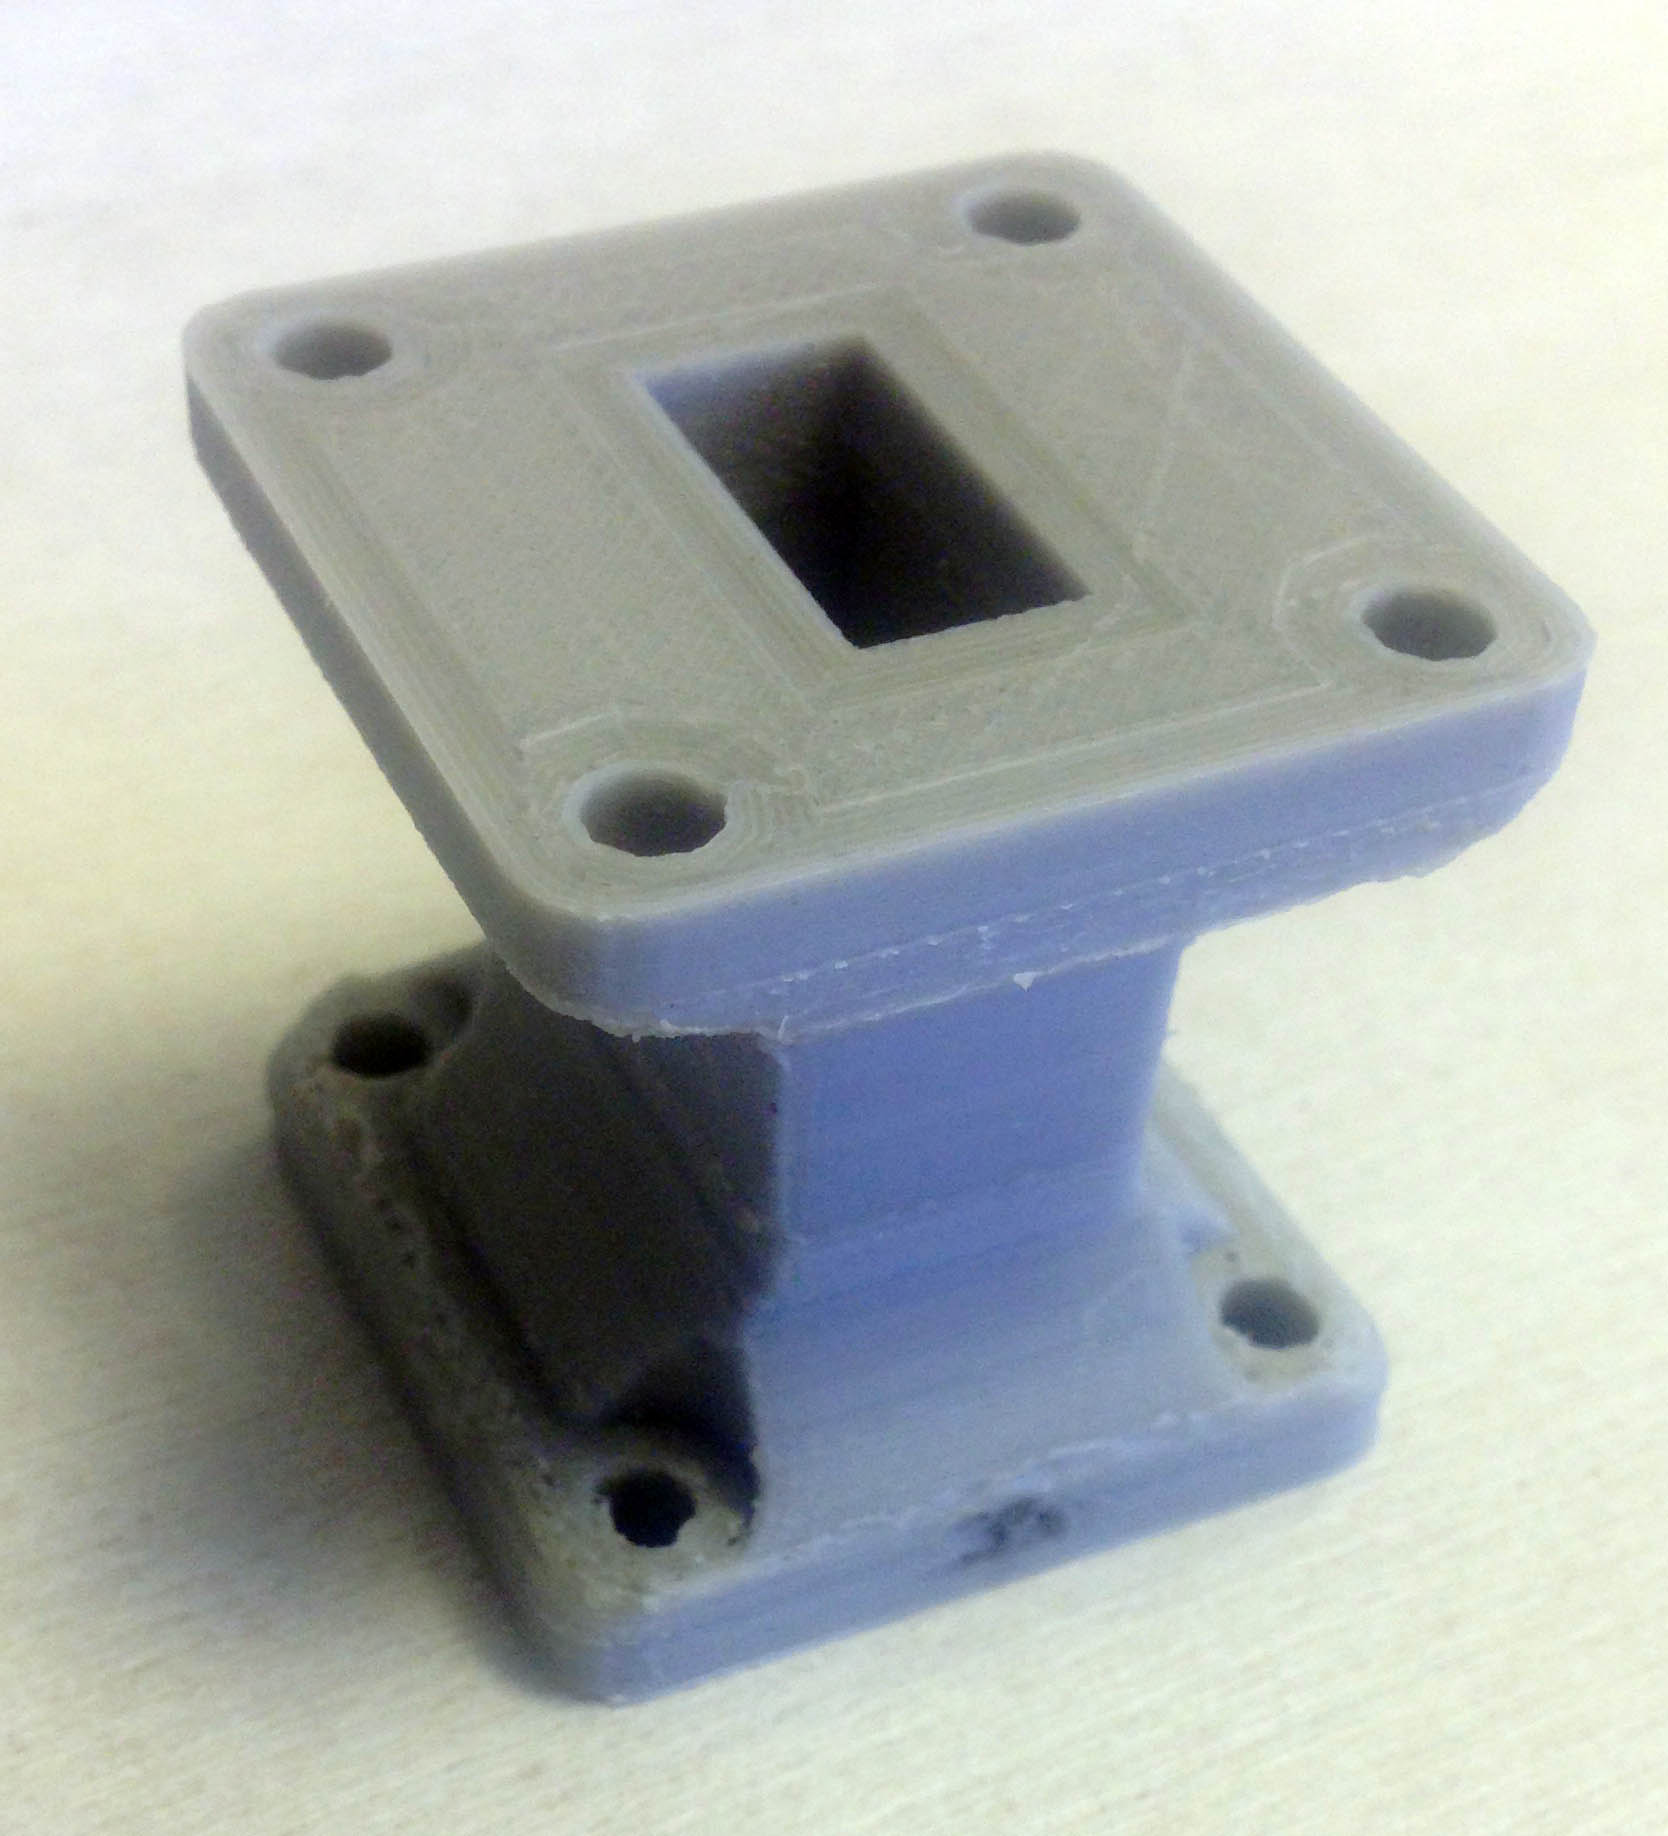
\includegraphics[height=5cm]{Figs5//3_pumice.JPG}
		\end{minipage}
	}
    \subfigure[]{
    \begin{minipage}[t]{0.35\textwidth}
			\centering
			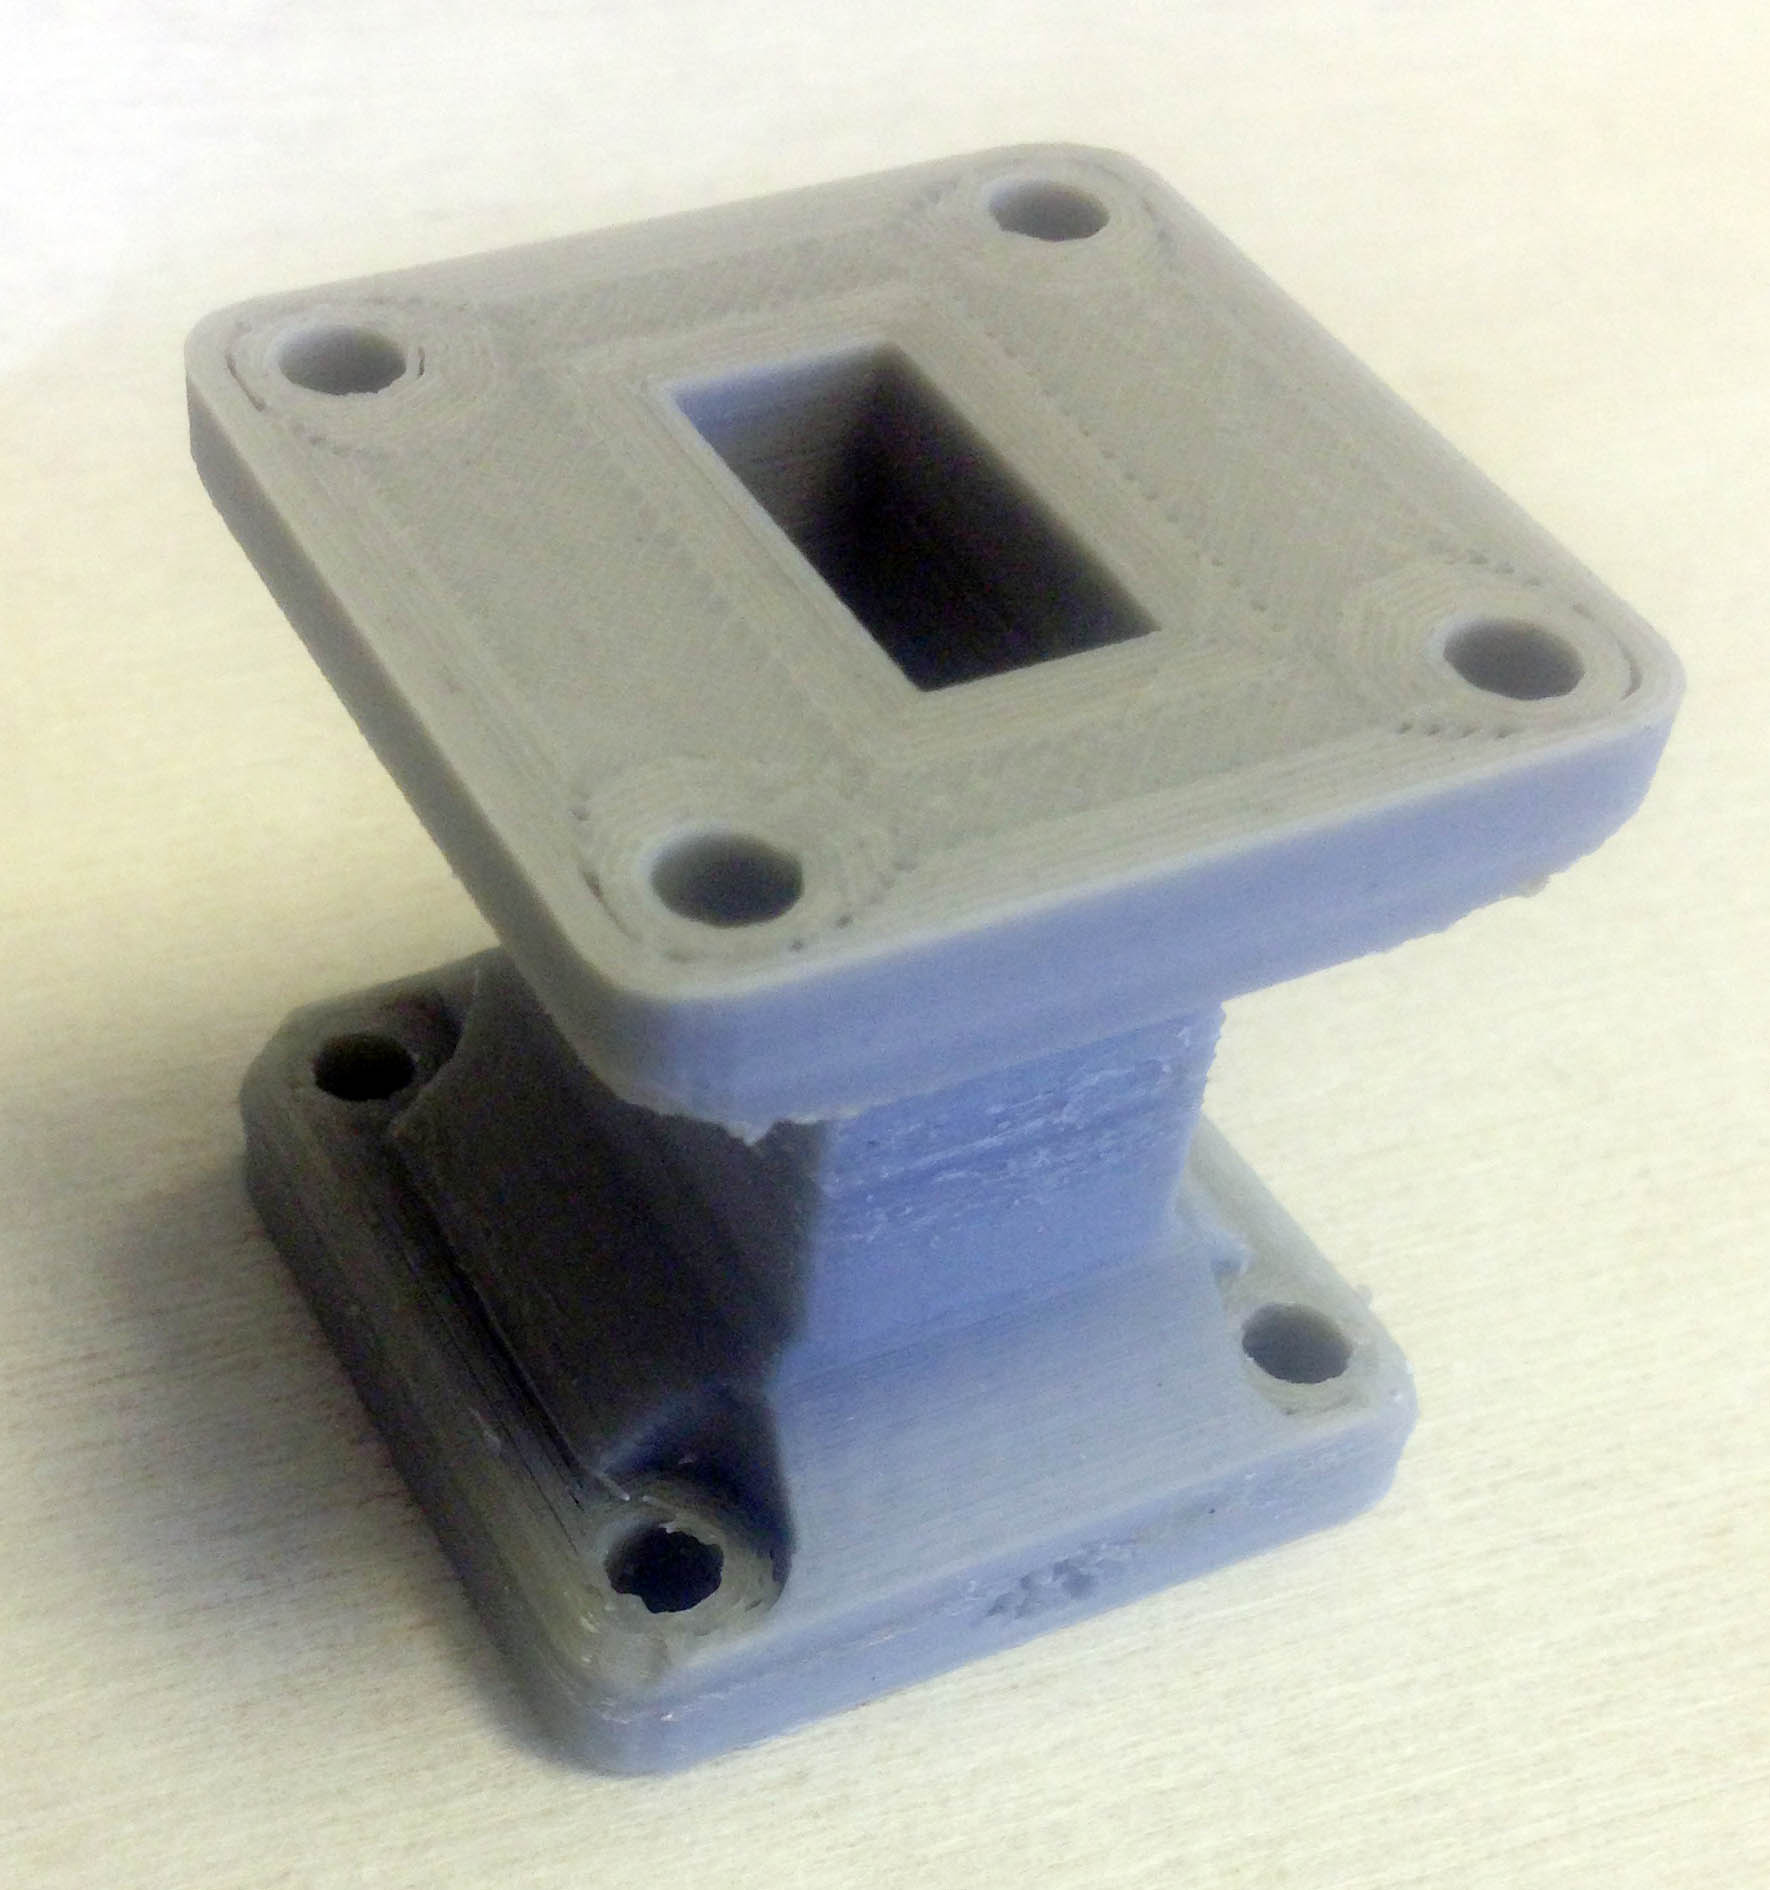
\includegraphics[height=5cm]{Figs5//4_pumice.JPG}
		\end{minipage}
	}
    \subfigure[]{
    \begin{minipage}[t]{0.35\textwidth}
			\centering
			\includegraphics[height=5cm]{Figs5//5_pumice.JPG}
		\end{minipage}
	}
    \subfigure[]{
    \begin{minipage}[t]{0.35\textwidth}
			\centering
			\includegraphics[height=5cm]{Figs5//6_pumice.JPG}
		\end{minipage}
	}
    \subfigure[]{
    \begin{minipage}[t]{0.35\textwidth}
			\centering
			\includegraphics[height=5cm]{Figs5//7_pumice.JPG}
		\end{minipage}
	}
  \caption[The 3D-printed waveguides]{\footnotesize The 3D-printed waveguides made of (a)no pumice, (b)1 wt.$\%$ pumice, (c)2 wt.$\%$ pumice, (d)3 wt.$\%$ pumice, (e)4 wt.$\%$ pumice, (f)5 wt.$\%$ pumice, (g)6 wt.$\%$ pumice, (h)7 wt.$\%$ pumice.}
  \label{Fig:waveguides}
\end{figure}

\section{Analysis}
\subsection{The distribution of the pumice powder in filament}

According to the bad performance of the filament containing 7 wt.\% pumice, the main reason is the air bubbles in the filament and its brittleness. The pumice powder could be seen with the microscope in Figure \ref{Fig:pumice}. Compared with the corresponding calibration, the size of pumice powder is between 2-12$\mu$m. From the microscope pictures of the filament, it is easy to find the small pumice particles. It is obvious that there is an air bubble in Figure\ref{Fig:slice} (b) with lots of pumice particles nearby. Based on these pictures, the distribution of the pumice powder in the filament is not uniform and the most of the powder is around the air bubbles. It could be deduced that the air bubble and the converge of pumice particles could make the filament very brittle and even block the nozzle head during printing.\\
\\
There is a high possibility that the air bubbles could be avoided in a very dry environment. It is necessary to use an oven to slightly melt ABS pellets and dry pumice powder rather than the coffee grinder. In order to distribute pumice powder evenly in the filament, the screw in extruder should be longer and multi-functional to mix the ABS and pumice sufficiently.
\begin{figure}[htbp] % make the image in the middle of paragraph
	\centering
    \subfigure[]{
    \begin{minipage}[t]{0.45\textwidth}
			\centering
			\includegraphics[height=5cm]{Figs5//pumi.jpg}
		\end{minipage}
	}
    \subfigure[]{
    \begin{minipage}[t]{0.45\textwidth}
			\centering
			\includegraphics[height=5cm]{Figs5//calibration.jpg}
		\end{minipage}
	}
  \caption{The microtexture of the pumice powder}{\footnotesize (a)pumice powder (b)corresponding calibration }
    \label{Fig:pumice}
\end{figure}

\begin{figure}[htbp] % make the image in the middle of paragraph
	\centering
    \subfigure[]{
    \begin{minipage}[t]{0.45\textwidth}
			\centering
			\includegraphics[height=5cm]{Figs5//ABS.jpg}
		\end{minipage}
	}
    \subfigure[]{
    \begin{minipage}[t]{0.45\textwidth}
			\centering
			\includegraphics[height=5cm]{Figs5//ABS7p.jpg}
		\end{minipage}
	}
  \caption[The microtexture of the filament]{\footnotesize The microtexture of the filament made by (a)pure ABS, (b)7 wt.$\%$ pumice and ABS. }
  \label{Fig:slice}
\end{figure}

\subsection{The measurement error of cubes}
From Table \ref{tab:cube density}, it is obvious that the measurement error is quite big. Therefore, the density calculated by this method is not reliable. The main reason behind it is the bad quality of the printed cubes. The geometrical accuracy of the cubes is quite high due to the warp of ABS. And the extruded filament is thinner than the printer supposes it to be so that there are some gaps between the layers. The cubes are not 100$\%$ filled inside which make the weight is lighter than the theoretical one. The effect of pumice powder is not only the brittleness actually. The filament made by pumice powder and ABS contains air inside and it is easier to absorb moisture from the environment than the pure ABS filament. And the average diameter of the filament is smaller than 2.85mm as the printer's default setting. In this case, the real volume of the printed material is less than our design of the model when the printer extrudes the specific length of the filament as the G-code commands. The more pumice powder in the filament, the worse quality of the prints. As for the density of the manufactured filament, the printability of the filament is sacrificed for the lighter weight of the filament since it contains air bubbles, which is not meaningful.

\subsection{The geometrical accuracy of waveguides}
The overall results indicate the pumice powder could improve the quality of prints when its weight percentage is lower than 6$\%$ according to the equipment facilitated in this project. Otherwise, it cannot be printable when the weight percentage of pumice powder is beyond 7\%. Focused on the inner wall flatness of the waveguides, the worst one is produced by 7 wt.$\%$ pumice. It is because the filament is too brittle to print with and the nozzle is easily blocked during the printing.

\begin{figure}[htbp] % make the image in the middle of paragraph
	\centering
	\subfigure[]{
    \begin{minipage}[t]{0.35\textwidth}
			\centering
			\includegraphics[height=5cm]{Figs5//in0.JPG}
		\end{minipage}
	}
	\subfigure[]{
		\begin{minipage}[t]{0.35\textwidth}
			\centering
			\includegraphics[height=5cm]{Figs5//in1.JPG}
		\end{minipage}
        }
        \subfigure[]{
    \begin{minipage}[t]{0.35\textwidth}
			\centering
			\includegraphics[height=5cm]{Figs5//in2.JPG}
		\end{minipage}
	}
        \subfigure[]{
    \begin{minipage}[t]{0.35\textwidth}
			\centering
			\includegraphics[height=5cm]{Figs5//in3.JPG}
		\end{minipage}
	}
    \subfigure[]{
    \begin{minipage}[t]{0.35\textwidth}
			\centering
			\includegraphics[height=5cm]{Figs5//in4.JPG}
		\end{minipage}
	}
     \subfigure[]{
    \begin{minipage}[t]{0.35\textwidth}
			\centering
			\includegraphics[height=5cm]{Figs5//in5.JPG}
		\end{minipage}
	}
    \subfigure[]{
    \begin{minipage}[t]{0.35\textwidth}
			\centering
			\includegraphics[height=5cm]{Figs5//in6.JPG}
		\end{minipage}
	}
    \subfigure[]{
    \begin{minipage}[t]{0.35\textwidth}
			\centering
			\includegraphics[height=5cm]{Figs5//in7.JPG}
		\end{minipage}
	}
  \caption[The inner wall of the waveguides]{\footnotesize The inner wall of the waveguides made by (a)no pumice, (b)1 wt.$\%$ pumice, (c)2 wt.$\%$ pumice, (d)3 wt.$\%$ pumice, (e)4 wt.$\%$ pumice, (f)5 wt.$\%$ pumice, (g)6 wt.$\%$ pumice, (h)7 wt.$\%$ pumice.}
  \label{Fig:inner}
\end{figure}


